\documentclass[output=paper,modfonts,nonflat]{langsci/langscibook} 
\ChapterDOI{10.5281/zenodo.2579047}

\title{Extracting and aligning multiword expressions from parallel corpora} 

\author{Nasredine Semmar\affiliation{CEA LIST, Vision and Content Engineering Laboratory}\and Christophe Servan\affiliation{University of Grenoble Alpes -- Grenoble Informatics Laboratory\\ SYSTRAN}\and Meriama Laib\affiliation{CEA LIST, Vision and Content Engineering Laboratory}\and Dhouha Bouamor\affiliation{Actimos, Groupe Accord}\lastand  Morgane Marchand\affiliation{eXenSa}}

\lehead{N. Semmar, C. Servan, M. Laib, D. Bouamor \& M. Marchand}
%\shorttitlerunninghead{}

% \epigram{}

\abstract{Bilingual lexicons of multiword expressions play a vital role in several natural language processing applications such as machine translation and cross-language information retrieval because they  often characterize domain-specific vocabularies. Word alignment approaches are generally used to construct bilingual lexicons automatically from parallel corpora. We present in this chapter three approaches to align multiword expressions from parallel corpora. We evaluate the bilingual lexicons produced by these approaches using two methods: a manual evaluation of the alignment quality and an evaluation of the impact of this alignment on the translation quality of the phrase-based statistical machine translation system Moses. We experimentally show that the integration of the bilingual lexicons of multiword expressions in the translation model improves the performance of Moses.
}

\begin{document}
\maketitle

% Introduction
\section{Introduction}

A MultiWord Expression (MWE) is a combination of words for which syntactic or semantic properties of the whole expression cannot be obtained from its parts \citep{sag02}. Such units could be collocations, compound words, named entities, etc. They constitute an important part of the lexicon of any natural language \citep{jackendoff1997architecture}. Bilingual lexicons of MWEs play a vital role in several Natural Language Processing (NLP) applications such as Machine Translation (MT) and Cross-Language Information Retrieval (CLIR) because they generally characterize domain-specific vocabularies. The manual construction of these lexicons is often costly and time consuming. Word \isi{alignment} approaches are generally used to automatically construct bilingual lexicons from parallel or comparable corpora. Several \isi{word alignment} approaches have been explored \citep{daille1994towards,blank2000terminology,barbu2004} and many automatic \isi{word alignment} tools are available, such as GIZA++ \citep{och2000improved}. However, most of these tools are efficient only to align single words \citep{fraser2007measuring}.

The chapter is organized as follows. We survey in Section 2 previous works addressing the tasks of extracting and aligning MWEs from \isi{parallel corpora}. We define in Section 3 the notion of MultiWord Expression and describe different types of MWEs with examples.  In Section 4, we introduce three approaches to build bilingual lexicons of MWEs from sentence aligned \isi{parallel corpora}. The experimental results are reported and discussed in Section 5. Finally, we present in Section 6 the conclusion and future work.

% Related work
\section{Related work}

There are mainly two strategies to extract bilingual MWEs from \isi{parallel corpora}. The first strategy consists to acquire translations of phrases from \isi{parallel corpora} in one step. Phrases are not necessarily MWEs, they can be contiguous sequences of a few words that encapsulate enough context to be translatable \citep{denero2008complexity}. The second strategy firstly, identifies monolingual MWE candidates and then applies \isi{alignment} approaches to find bilingual correspondences \citep{daille1994towards,blank2000terminology,gaussier2011modeles,barbu2004}. 

In the second strategy, MWEs extraction can be processed by using symbolic methods based on morpho-syntactic patterns, or, though statistical approaches, which use automatic measures to rank MWE candidates. Finally, MWEs extraction can be done by using hybrid approaches, which combine the two first strategies.

\cite{dagan1994termight} proposed to use syntactic analysis to extract terminology. MWEs are extracted by grouping linguistically related terms. In the same way, \cite{okita2010multi} proposed to link across two languages MWEs according to their syntactic and lexical information. \cite{tufis2007parallel} and \cite{seretan2007collocation} introduce a linguistic approach in which they claim that MWEs keep in most cases the same morpho-\isi{syntactic structure} in the source and target languages.

Statistical approaches also have proven to be useful in collecting bilingual MWEs from \isi{parallel corpora}. \cite{kupiec1993algorithm} introduced the use of machine learning algorithms such as the Expectation Maximization (EM) to extract MWEs. Similarly, \cite{vintar2008harvesting} proposed to extract bilingual MWEs by translating MWEs from a well known language (\ili{English}) to a low resource language (Slovene) by using machine translation. They have shown that their translation-based approach performs better than using linguistic approaches. But they did not combine these two kind of approaches. The combination of such approaches enables to extract finer MWEs \citep{daille2001extraction}. In this way \cite{wu2003bilingual} and later \cite{boulaknadel2008multiterm}, proposed to use syntactic and statistical analysis to extract bilingual MWEs from a parallel corpus. The main aspect of their approach is a monolingual parsing to extract MWEs combined with statistical detection in each language, then, they confront candidates from each side to find bilingual MWEs.

Other approaches proposed to use machine translation to translate MWEs candidates found with a syntactic analysis \citep{seretan2007collocation}. Again, the first step is done on each language independently and then, a second step aims to match candidates across languages.

% \isi{Multiword Expressions}
\section{Multiword expressions}
In NLP, a multiword expression  refers to a non-composi\-tional sequence of words whose exact and unambiguous meaning, connotation and syntactic properties cannot be derived from the meaning or connotation of its components \citep{choueka1988looking,sag02}.
MWEs are frequently used in written texts and constitute a significant part of the language lexicon.

\cite{jackendoff1997architecture} considers that the frequency of their use is equivalent to that of single words.
Although MWEs are easily computed, stored and used by humans, their identification is a major issue for different type of NLP applications, namely for syntactic analysis \citep{nivre2004multiword,constant2011integrer}, automatic summarization \citep{hogan2007exploiting}, information extraction \citep{vechtomova2005role} and especially for machine translation and cross-language information retrieval \citep{carpuat2010task,ren2009improving}.

\subsection{Multiword expressions typology}

In the literature, MWEs are presented under different names or classifications such as \isi{idioms}, lexicalized phrases or collocations and several authors \citep{ramisch2013introduction} give a list of examples instead of giving an exact description of them.
According to \cite{calzolari2002}, MWEs are ``different but related phenomena'' and ``At the level of greatest generality, all of these phenomena can be described as a sequence of words that acts as a single unit at some level of \isi{linguistic analysis}''.

\cite{sag02} classify them into two main categories: lexicalized phrases and institutionalized phrases (Figure~\ref{sem:fig:TypoMWE}).
Lexicalized phrases ``have at least partially idiosyncratic syntax or semantics, or contain ``words'' which do not occur in isolation''.
Institutionalized phrases are ``semantically and syntactically compositional, but statistically idiosyncratic''.

\begin{figure}
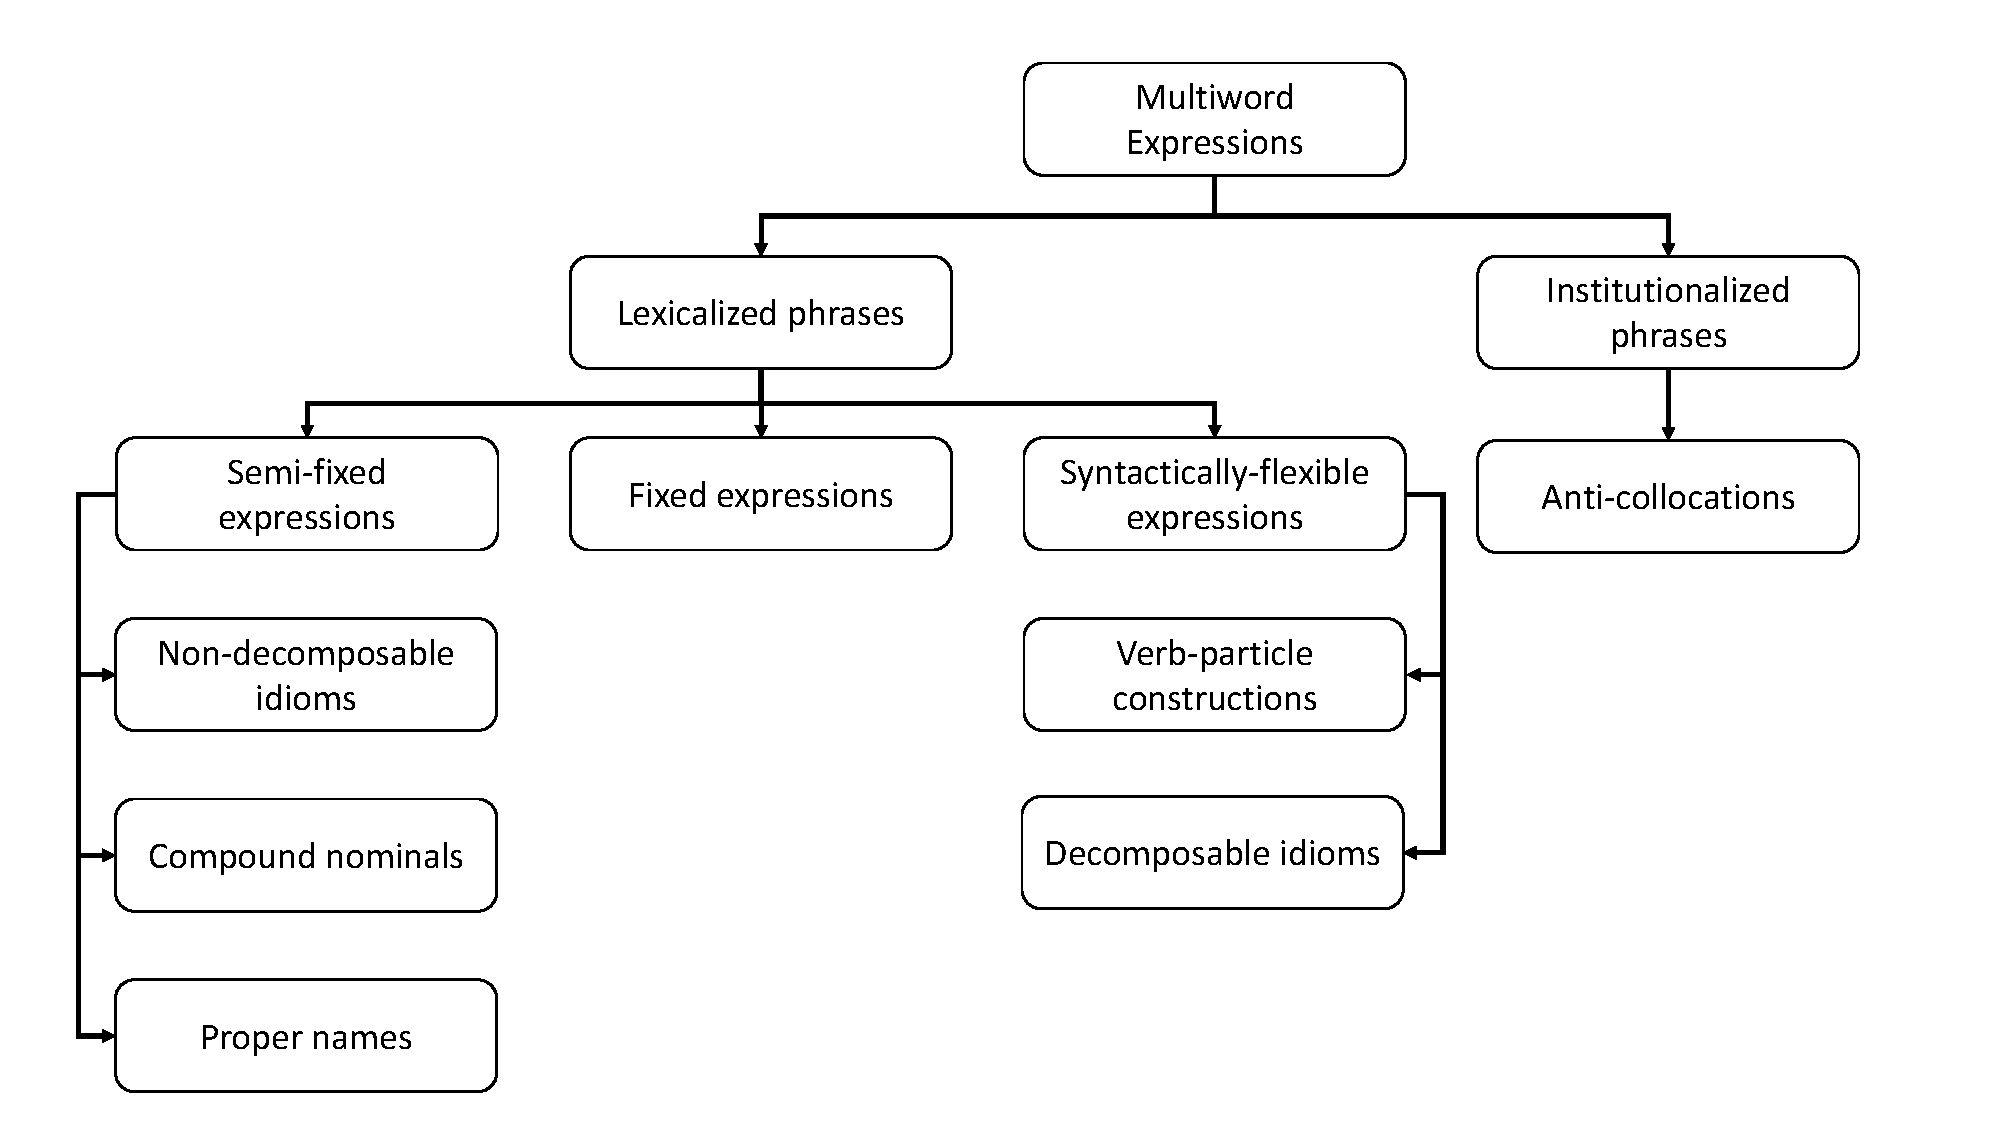
\includegraphics[width=\linewidth]{figures/figureTypologyMWE_NB.pdf}
\caption{\label{sem:fig:TypoMWE}Typology of multiword expressions by \cite{sag02}}
\end{figure}

\subsubsection{Lexicalized phrases}
In a decreasing order of lexical rigidity, these MWEs are broken down into three classes: \isi{fixed expressions}, semi-\isi{fixed expressions} and syntactically-flexible expressions.

\subsubsubsection{Fixed expressions}
Fixed expressions are non-compositional sequences of words.
They are syntactically and morphologically rigid and undergo neither internal modification nor morphological and syntactical \isi{variations} (e.g. ``nest of vipers'' in \ili{English} or ``pom\-me de terre'' in  \ili{French}).
To determine whether or not a sequence of words is a fixed expression, we can use linguistic criteria such as using synonyms or adding words between its components (cf. ``nest of many black vipers'' in \ili{English} or ``pomme de jolie terre lointaine'' in \ili{French}).
Fixed expressions can be considered as single entries in the dictionary.

\subsubsubsection{Semi-fixed expressions}
A semi-fixed expression is a non-compositional sequence of words whose components do not contribute to its figurative meaning.
Semi-\isi{fixed expressions} should respect a strict word order and some of them undergo limited lexical and morphological variability such as inflection and some variation in the reflexive form.
According to their characteristics, they can be broken down into three basic categories: non-decomposable \isi{idioms}, proper names and some compound nominals \citep{sag02}.

Non-Decomposable Idioms do not undergo syntax variability but their components accept lexical changes such as pronominal reflexivity form (e.g. ``wet himself'', ``wet themselves''), verbal inflection (``kick the bucket'', ``kicked the bucket'') or \isi{passivization} (e.g. ``briser le silence'' or  ``le silence est brisé'' in \ili{French}).
Proper Names ``are syntactically highly idiosyncratic'' \citep{sag02}.
They can be complex with two or three proper names as components, including person, places and organization names.

Compound Nominals are syntactically unalterable and undergo number inflection (e.g. ``car park(s)'' in \ili{English} or ``pomme(s) de terre'' in \ili{French}).

\subsubsubsection{Syntactically-flexible expressions}

Unlike semi-\isi{fixed expressions}, syntactically-flexible expressions undergo a wide degree of syntactic variation such as passivation (e.g., ``The cat was let out of the bag'') and allow external elements to intervene between their components (e.g., ``slow the car down''). This type of expressions includes \isi{verb-particle constructions}, decomposable \isi{idioms}. 
Particle verbs constructions are made up of a verb whose meaning is modified by one or more particles. They can be either semantically idiosyncratic such as ``brush up on''  or compositional such as ``take after'', ``look out'', ``go back'' and ``run over''.
Decomposable \isi{idioms} tend to be syntactically flexible to some degree that is unpredictable \citep{riehemann01}. Semantically, they behave as if their components were linked parts contributing independently to the figurative interpretation of the expression as a whole.

\subsubsection{Institutionalized phrases}
Institutionalized phrases are semantically and syntactically fully compositional, but statistically idiosyncratic \citep{sag02}. They occur in a high frequency and their idiosyncrasy is statistical rather than linguistic. They generally allow one available meaning. Institutionalized phrases often refer to “collocations” \citep{barz1996komposition,riehemann01,burger2010phraseologie}, described as sequences of words that statistically have a high probability to appear together whether they are contiguous or not (e.g., ``make love'' or ``make a difference'').

% Construction of bilingual lexicons of MWEs from \isi{parallel corpora}
\section{Construction of bilingual lexicons of MWEs from parallel corpora}


In this section, we describe three approaches to build bilingual lexicons of MWEs from a
sentence aligned parallel corpus. The first two approaches are composed of two steps. The first step identifies MWEs present in the parallel corpus, and the second step establishes correspondence relations between the MWEs of the source text and their translations in the target text. The third approach performs the terminology extraction and \isi{alignment} tasks in one step. 

% Statistical approach for \isi{MWE alignment}
\subsection{Statistical approach for MWEs alignment}

The statistical approach for MWEs \isi{alignment} consists first in identifying the relevant word groups through the use of $n$-gram statistics in both the source and target languages. 
Then for each source MWE extracted we compile a list of candidate translations through the use of two distance metrics. 
The list of candidates is then pruned through the use of heuristics like the length of each MWE, and a translation is ``found'' if it satisfies confidence threshold on the distance metric and the heuristics.

The \isi{alignment} process has the following four steps \citep{semmar2010hybrid}:
\begin{enumerate}
 \item Monolingual extraction of MWEs: The role of this step consists to identify all the $n$-grams (up to 6-grams) that may represent a MWE. This is done through frequency analysis and heuristic scoring. This step outputs two lists of terms, which we will refer to as SC (MWE in the Source Language) and TC (MWE in the Target Language).
 \item Frequency distance calculation: This step calculates for all source MWEs in SC the distance to each of the target MWEs in TC. The main idea of this metric is that if two MWEs are translations of each other then they must appear together in the corpus segments, and only together. Their frequency distance is then calculated as follows:
 \begin{equation}
  FD(s,t)=\frac{|f(s)-f(t)|}{\max(f(s),f(t))}
 \end{equation}
 Where, $f(s)$ is the frequency of the source MWE and $f(t)$ is the frequency of the target MWE under consideration.

We observe that if $T$ is the translation of $s$, $f(s) = f(t) $ then we have distance equal to 0. 
Also, if two MWEs always occur together but one is much more frequent than the other, the distance could have a value other than 0 and they would not be considered translations of each other. 
Here we chose to apply a threshold of 0.25 as the maximum allowable distance. This threshold is calculated empirically and can be tuned to achieve better precision.

\item Co-occurrence distance ($CD$): The previous step only considers frequencies so it may be possible for two completely unrelated MWEs to achieve a low distance score. To refine extraction results, we also check for a co-occurrence score as follows:
\begin{equation}
  CD(X,Y)=\frac{\sqrt{\sum(X_i-Y_i)^2}}{N}
\end{equation}
Where, $X_i$ is the number of occurrences of $s$ in the $i^{th}$ \isi{segment} of the SL, $Y_i$ is the number of occurrences of $t$ in the $i^{th}$ \isi{segment} of the $TL$ and $N$ is the number of segments.

This check allows the rejection of the MWEs that fortuitously have similar frequency. Since they would not appear in the same segments, the terms $X_i-Y_i$ would increase. The candidate list can be ordered through $CD$.

\item Pruning MWEs candidates: After obtaining an ordered list of target MWEs candidates, we remove:
\begin{itemize}
 \item The candidates which have a length different from the source MWE;
 \item The candidates which have been previously aligned with another source MWE and where the co-occurrence score was better.
\end{itemize}
\end{enumerate}

Because of the statistical nature of this approach, it performs much better for MWEs that occur often in the corpus. Table~\ref{sem:MWEexamples} illustrates some MWEs and their translations extracted from the bi-sentence “Approval of the Minutes of the previous sitting/Approbation du procès-verbal de la séance précédente”. It should be noted that before applying the MWEs \isi{alignment} approach, we lemmatize the parallel corpus. This lemmatization is achieved using the CEA LIST Multilingual Analyzer LIMA  \citep{besancon2010}.

\begin{table}
\caption{Some examples of aligned MWEs with the statistical approach}
\label{sem:MWEexamples}
 \begin{tabular}{ll} 
  \lsptoprule
            \ili{English} MWE& \ili{French} MWE \\ 
  \midrule
minute & procès-verbal \\
approval of the minute & approbation du procès-verbal \\
previous sitting & séance précédent \\
  \lspbottomrule
 \end{tabular}
\end{table}

% Hybrid approach for \isi{MWE alignment} using morpho-syntactic patterns
\subsection{Hybrid approach for MWEs alignment based on morpho-syntactic patterns} 
The hybrid approach for MWEs \isi{alignment} is composed of the following two steps \citep{bouamor2012study,bouamor2012identifying,bouamor2012automatic}:
\begin{enumerate}
 \item MWEs identification: The method used to extract MWEs is based on a symbolic approach relying on morpho-syntactic patterns.
\item MWEs \isi{alignment}: After extracting MWE candidates, context vectors from the parallel corpus are separately built and similarity scores between one MWE and all target MWEs are computed.
\end{enumerate}

\subsubsection{MWEs extraction}

The method to extract monolingual MWEs from a parallel corpus is based on a symbolic approach relying on morpho-syntactic patterns. 
It handles both frequent and infrequent expressions and do not use any lexicon. This method involves a full morpho-syntactic analysis of source and target texts. 
The analysis is done using the CEA LIST Multilingual Analysis platform LIMA \citep{besancon2010}, which produces Part-of-Speech (POS) tags and lemmas associated to each word. Since most MWEs consist of noun, adjectives and prepositions, we adopted a linguistic filter. 
It consists in keeping only $n$-gram ($n$ from 2 to 4) units, which match with a list of a hand created morpho-syntactic patterns. 
Such process is used to keep only specific strings and filter out undesirable ones such as candidates composed mainly of stop words (``of a, is a, that was''). 
The algorithm operates on lemmas instead of surface forms which can draw on richer statistics and overcome the data sparseness problems. 

In Table~\ref{sem:MWEexamplespatterns}, we give an example of MWEs produced for each pattern. There exists extraction patterns (or configurations) for which no MWE has been generated (i.e., Noun-Adj). 
To this list are added some prepositional idiomatic expressions (``in particular'', ``in the light of'', ``as regards'', etc.) and named entities (``Middle East'', ``South Africa'', ``United States of America'', etc.) recognized by the morpho-syntactic analyzer LIMA. 
Then, we scored all extracted MWEs with their total frequency of occurrence in the corpus. To avoid an over-generation of MWEs and remove irrelevant candidates from the process, a redundancy cleaning approach is introduced.
In this approach, if a MWE is nested in another, and they both have the same frequency, we discard the smaller one. Otherwise we keep both of them. We consider also the case in which a MWE appears in a high number of terms and discard all longer ones. 

Our approach does not use any additional correlations statistics such as Mutual Information or Log Likelihood Ratio. It finds translations for all extracted MWEs (both frequent and infrequent ones).

\begin{table}
%\scriptsize
\centering
\caption{Example of morpho-syntactic patterns used to detect MWEs in each language independently}
\label{sem:MWEexamplespatterns}
 \begin{tabular}{lll} 
  \lsptoprule
            pattern & \ili{English} MWE & \ili{French} MWE \\ 
  \midrule
            Adj-Noun & plenary meeting & libre circulation\\ 
            Noun-Noun & member state & état membre \\
            Noun-Prep-Noun & point of view & point de vue \\
            Noun-Prep-Adj-Noun & court of first instance & court de première instance \\
    \lspbottomrule
 \end{tabular}
\end{table}



\subsubsection{MWEs alignment}
MWEs \isi{alignment} aims to find for each MWE in a source language its adequate translation in the target one. 
This task used to be handled through an external linguistic resource such as bilingual lexicons or single words \isi{alignment} tools. Our approach for MWEs \isi{alignment} is resource-independent and uses a parallel corpus and a list of input MWEs candidates to translate. It associates a specific representation to each expression (source and target). 

We associate to each MWE an \textit{N} sized vector, where \textit{N} is the number of sentences in the corpus, indicating whether it appears or not in each sentence of the corpus. 
Our algorithm is based on the Vector Space Model \citep{salton1975vector}.
This vector space representation will serve, eventually, as a basis to establish a translation relation between each pair of MWEs. 
 
To extract translation pairs of MWEs, we propose an iterative \isi{alignment} algorithm operating as follows:
\begin{enumerate}
\item Find the most frequent MWE \textit{exp} in each source sentence;
\item Extract all target translation candidates, appearing in all parallel sentences to those containing \textit{exp};
\item Compute a confidence value $V_{Conf}$ for each translation relation between \textit{exp} and all target translation candidates;
\item Consider that the target MWE maximizing $V_{Conf}$ is the best translation;
\item Discard the translation pair from the process and go back to 1.
\end{enumerate}

To compute the confidence value $V_{Conf}$, we adopted the $\mathit{Jaccard}$ Index. % (see equation~\ref{sem:jaccard}).
This measure is based on the number $I_{st}$ of sentences shared by each target and a source MWE. 
$I_{st}$ is normalized by the sum of the number of sentences where the source and target MWEs appear independently of each other (respectively $V_s$ and $V_t$) decreased by $I_{st}$. 
 \begin{equation}
 \label{sem:jaccard}
  \mathit{Jaccard}=\frac{I_{st}}{V_s+V_t-I_{st}}
 \end{equation}


We illustrate in Table~\ref{sem:MWEexamplesalignements}, a sample of aligned MWEs by means of the algorithm described above.  When we observe MWE pairs, we noticed that our method has two advantages. On the one hand, it allows the translation of MWEs aligned in most previous work \citep{dagan1994termight,ren2009improving} using single words \isi{alignment} tools to establish word-to-\isi{word alignment} relations. 
The approach can capture the semantic equivalence between expressions such as ``insulaire en développement'' and ``small island developing'' in a different way.
 On the other hand, the approach enables the \isi{alignment} of \isi{idioms} such as ``à nouveau'' (once more). 

%\begin{table}
%\caption{Some examples of aligned MWEs with the hybrid approach.}
%\label{sem:MWEexamplesalignements}
% \begin{tabular}{cc} 
%  \lsptoprule
%         \multicolumn{2}{c}{\ili{English}$\rightarrow$\ili{French} MWEs}\\ 
%  \midrule
%            european parliament & parlement européen \\ 
%            military coup & coup d'état \\
%            in favour of &  en faveur de \\
%            no smoking area & zone non fumeur \\
%            small island developing & insulaire en développement \\
%            good faith & de bonne foi \\
%            competition policy & politique de concurrence \\
%            process of consultation & processus de consultation \\
%            railway sector & chemin de fer \\
%            with regard to & en ce qui concerne \\
%						once more & à nouveau \\
%            cut in forestation & coupe forestière \\
%  \lspbottomrule
% \end{tabular}
%\end{table}


\begin{table}
\caption{Some examples of aligned MWEs with the hybrid approach based on morpho-syntactic patterns}
\label{sem:MWEexamplesalignements}
 \begin{tabular}{lllll} 
  \lsptoprule
            \ili{English} MWE& \ili{French} MWE \\ 
  \midrule
						european parliament & parlement européen \\ 
            military coup & coup d'état \\
            in favour of &  en faveur de \\
            no smoking area & zone non fumeur \\
            small island developing & insulaire en développement \\
            good faith & de bonne foi \\
            competition policy & politique de concurrence \\
            process of consultation & processus de consultation \\
            railway sector & chemin de fer \\
            with regard to & en ce qui concerne \\
						once more & à nouveau \\
            cut in forestation & coupe forestière \\
  \lspbottomrule
 \end{tabular}
\end{table}

% \end{enumerate}

% Hybrid approach for \isi{MWE alignment} based on \isi{linear programming}
\subsection{Hybrid approach for MWEs alignment based on linear programming}
This section describes a hybrid approach combining linguistic and statistical information which performs terminology extraction and \isi{alignment} of MWEs from parallel texts in one step \citep{marchandhybrid2011}. 

Most of works on MWEs \isi{alignment} are divided in two tasks: a monolingual step in which candidate terms are extracted and a bilingual step in which these terms are aligned with their translations \citep{gaussier2011modeles}. Word \isi{alignment} techniques are generally used to achieve the bilingual step. These approaches in multiple steps have the disadvantage to potentially propagate errors.

The main idea of the hybrid approach for MWEs \isi{alignment} based on \isi{linear programming} is to consider the global task of selection and \isi{alignment} as an optimization problem. 
The challenge when we deal with \isi{alignment} of MWEs is the exponential complexity of such a task. 
The possible number of fragments in a sentence improves exponentially according to the number of the words of the sentence. 
Several works impose some constraints on the number of fragments of a MWE. 
In our approach, the only restriction we made on MWEs is contiguity. The advantage to assume the continuity is to enable a linearized formulation of the optimization problem to solve. We use an integer \isi{linear programming} approach inspired by the work described in \citet{denero2008complexity} to quickly find an approximated optimal solution.

\subsubsection{Linear programming model}

A sentence pair consists of two word sequences: $e$ and $f$. 
$e_{ij}$ is the MWE from between-word positions $i$ to $j$ of $e$. 
$f_{kl}$ is the same for $f$. 
A link is an aligned pair of MWEs, denoted $(e_{ij},f_{kl})$. 
Each $e_{ij}$ is allowed to be linked with several $f_{kl}$ and each $f_{kl}$ with several $e_{ij}$. 
An \isi{alignment} $a$ of the sentence pair $(e,f)$ is a segmentation of the two sentences in MWEs with the set of links between these MWEs.
We use a real-valued function $\phi:\{e_{ij}\}\times\{f_{kl}\}\rightarrow R$ to score links. 
The score of an \isi{alignment} is then the product of all the links inside it:

\begin{equation}
\phi(a)=\prod_{(e_{ij},f_{kl})\in a} \phi(e_{ij},f_{kl})
\end{equation}

\begin{figure}
  %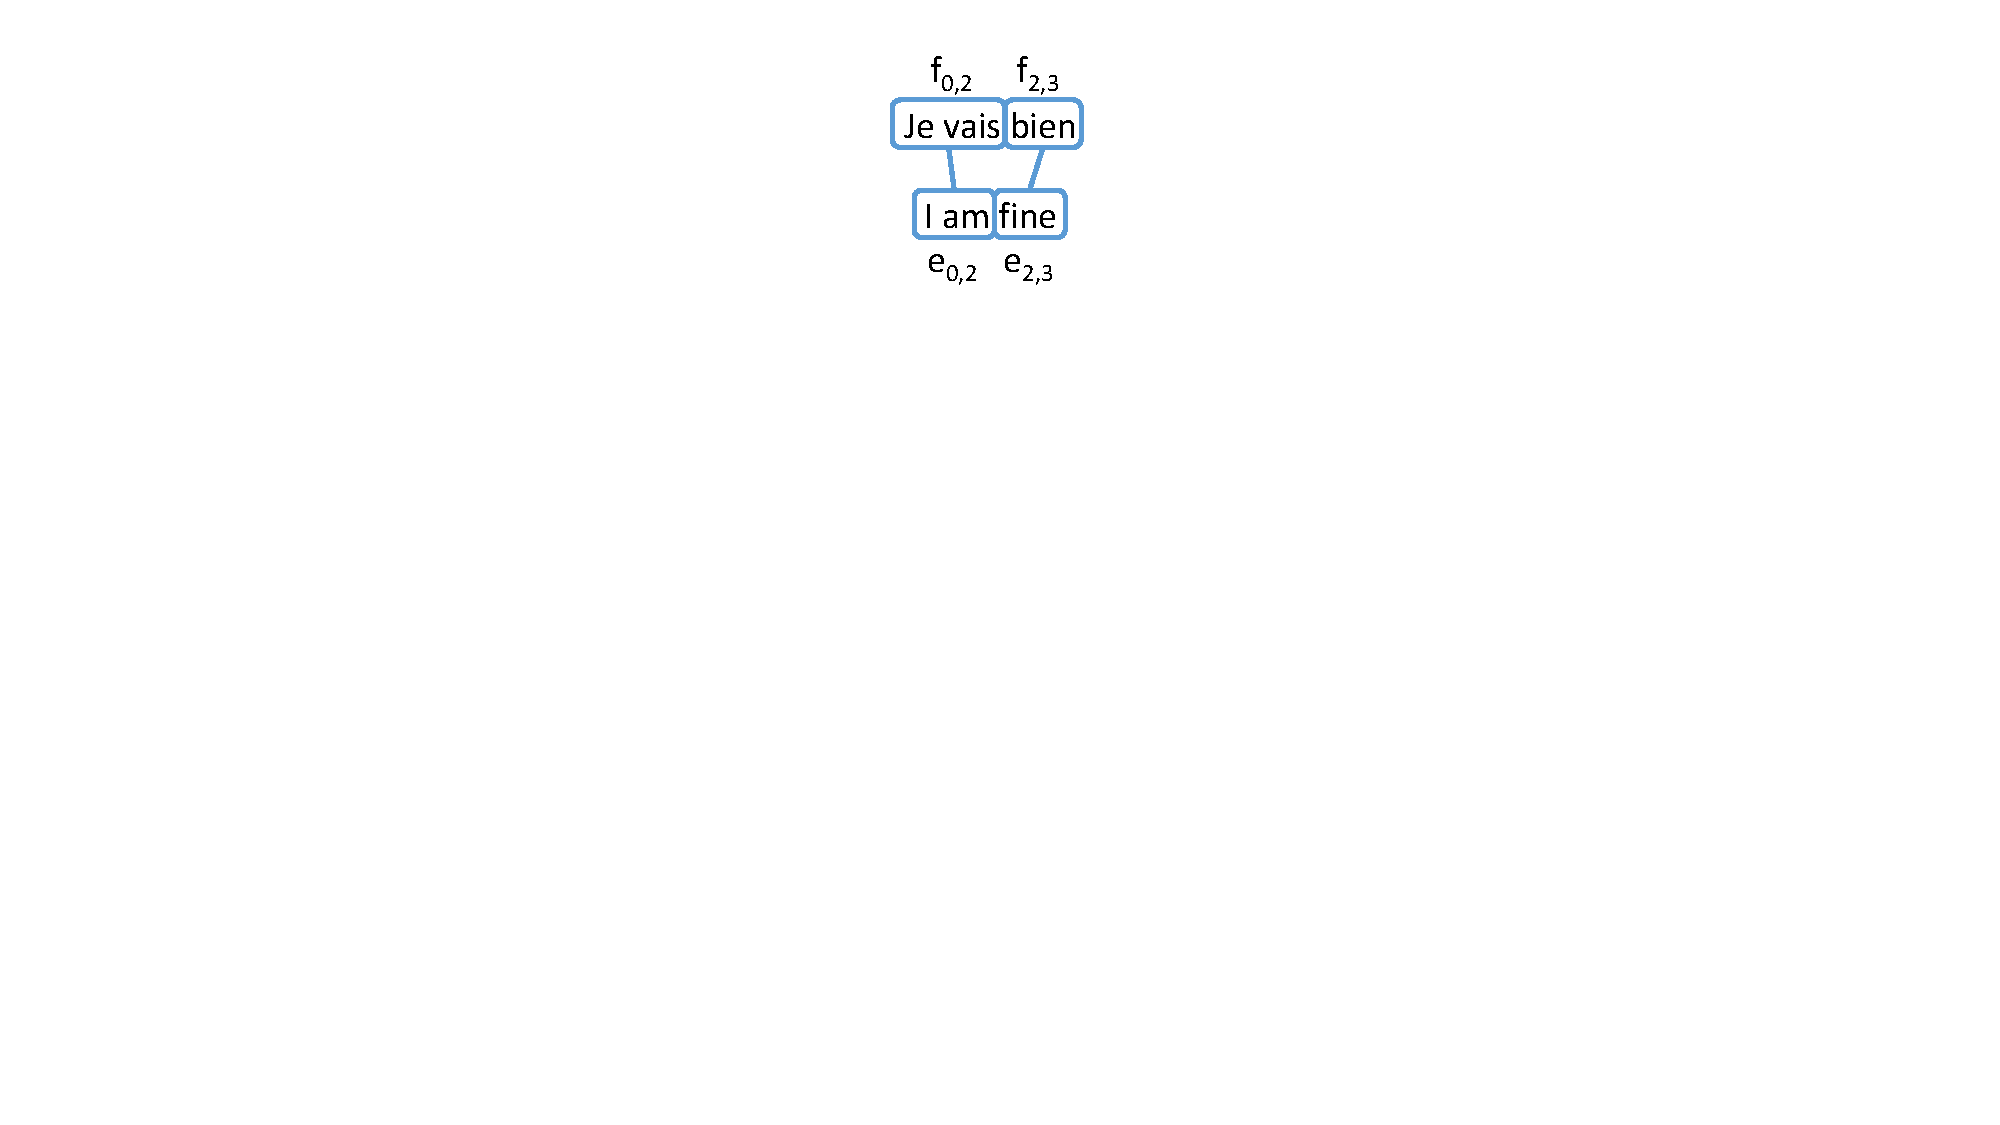
\includegraphics[width=3cm]{figures/Figure_exempleAli}
  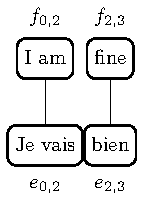
\includegraphics[scale=1.]{figures/figExSem}
\caption{\label{sem:fig:aliEx}Example of alignment}
\end{figure}


In the example shown in Figure~\ref{sem:fig:aliEx}, the score of the \isi{alignment} is computed as follows:
\begin{equation}
\phi(a)=\phi(e_{0,2},f_{0,2}) \times \phi(e_{2,3},f_{2,3})
\end{equation}

Formally this function has no constraints other than that of being real. 
In practice, we choose a function that gives an idea about the relevance to align such fragments. 
The higher the score, the higher the relevance of \isi{alignment} is important. 
Therefore, we look for the \isi{alignment} (segmentation + links) that maximizes the score described above.

First, we introduce binary variables $A_{i,j,k,l}$ denoting whether $(e_{ij},f_{kl}) \in a$.
Furthermore, we introduce binary indicators $E_{i,j}$ and $F_{k,l}$ that denote whether some $(e_{ij} ,  \cdotp)$ or $( \cdotp, f_{kl})$ appears in \textit{a}, respectively. 
Finally, we will use $W_{i,j,k,l} = log \phi(e_{ij},f_{kl})$ to transform the product into a sum.
When optimized\footnote{We used the open source solver GLPK (GNU Linear Programming Kit), available at \url{http://www.gnu.org/s/glpk/}.}, the integer program yields the optimal \isi{alignment}:

% Début formule
\begin{equation}
	\begin{cases}
	    \max \sum\limits_{i,j,k,l}{W_{i,j,k,l}A_{i,j,k,l}}\\
	    \\
	    \forall~x: 1\leq x\leq |e| & \sum\limits_{i,j: i<x\leq j}{E_{i,j}} = 1 \hspace{1.3cm}(1)\\
	    \forall~y: 1\leq y\leq |f| & \sum\limits_{k,l: k<y\leq l}{F_{k,l}} = 1 \hspace{1.3cm}(2)\\
	    \forall~i,j & \sum\limits_{k,l}{A_{i,j,k,l}} \geq E_{i,j} \hspace{1.2cm}(3)\\
	    \forall~k,l & \sum\limits_{i,j}{A_{i,j,k,l}} \geq F_{k,l} \hspace{1.2cm}(4)\\
	    \forall~i,j,k,l & 2\cdot A_{i,j,k,l} \leq E_{i,j}+F_{k,l} \hspace{0.3cm}(5)\\
	\end{cases}\\
\end{equation}
	With the following constraints:
\begin{equation}
	\begin{cases}
	0 \leq i < |e|, & 0 < j \leq |e|, \hspace{0.3cm} i < j\\
	0 \leq k < |f|, & 0 < l \leq |f|, \hspace{0.3cm} k < l\\ 
	\end{cases}\\
\end{equation}
% Fin formule

Constraints (1) and (2) indicate that a word is inside exactly one \isi{phrase}. Constraint (3) ensures that each \isi{phrase} in the selected partition of $e$ appears in at least one link (and likewise \isi{constraint} (4) for $f$). Finally, \isi{constraint} (5) ensures that if a link exists between $e_{ij}$ and $f_{kl}$ (i.e. $A_{i,j,k,l}=1$) then $e_{ij}$ and $f_{kl}$ are in the selected partitions of $e$ and $f$.

In that way, our approach differs from the one proposed in \citet{denero2008complexity}. 
Their work focuses on bijective alignments while we consider surjective alignments. 
We have also modified constraints (3) and (4) and added \isi{constraint} (5) to allow a \isi{phrase} to be aligned with several other phrases. 
We have chosen this formalism because phrases are not necessarily composed of contiguous words.

This integer program can work with any real-valued scoring function.

\subsubsection{Co-occurrence based metric}

We use a corpus aligned sentence-by-sentence to compute co-occurrence distance. For each MWE, we consider the presence or absence in each sentence. Then the score between two MWEs $e_{ij}$ and $f_{kl}$ is calculated as follows:

\begin{equation}
\phi_c(e_{ij},f_{kl})=\frac{\sum\limits_{s'\in S} N_{s'}(e_{ij}) \times N_{s'}(f_{kl})}{\sum\limits_{s\in S} N_{s}(e_{ij}) + N_{s}(f_{kl}) - N_{s}(e_{ij}) \times N_{s}(f_{kl})}
\end{equation}

Where $N_{s}(e_{ij})$ is 1 if the \isi{phrase} $e_{ij}$ of the first language is present in the sentence $s$ of the corpus $S$ and $0$ otherwise. 
$N_{s}(f_{kl})$ is similar for the other language.

\begin{table}[h!]
\begin{tabular}{rcl}
  \lsptoprule
Je mange un \emph{avocat} & -- & I'm eating an \emph{avocado} \\
L'\emph{avocat} prend la parole & -- & The \emph{lawyer} takes the floor \\
  \lspbottomrule
\end{tabular}
\caption{\label{sem:tab:probtrans} Example of ambiguous translation of MWEs}
\end{table}
This score calculates the number of common presence of both phrases divided by the number of total presence of either \isi{phrase}. 
Note that if none of $e_{ij}$ or $f_{kl}$ appears in the whole corpus, the score is set to $0$. 
Indeed, if two MWEs appear exactly in the same bi-sentences, they are probably translation of each other and the score will be $1$. 
The example in Table~\ref{sem:tab:probtrans} illustrates this score.

In this small corpus, $N_1(avocat) = 1$, $N_1(avocado) = 1$, $N_2(avocat) = 1$ and $N_2(avocado) = 0$. Thus, the co-occurence score for the bi-gram "avocat/avocado" has the value:
\begin{equation}
\phi_{c}(avocado,avocat) = \frac{(1 \times 1) + (1 \times 0)}{(1 + 1 -1 \times 1) + (1 + 0 - 1 \times 0)} = \frac{1}{2}
\end{equation}

We observed after aligning some sentences that when both sentence structures are similar, the aligner performs well as shown in Figure~\ref{sem:fig:goodali}. The segmentation is word to word or MWE to MWE depending on what is more frequent in the corpus. Moreover, the surjective formulation of the problem allows us to begin to detect expressions in two parts. 
We can see that ``rôle'' is linked to both ``role'' and ``play'' (Figure 3, Alignment 3).

This would have been impossible with the bijective formulation of \citet{denero2008complexity}. This result is encouraging but not yet sufficient. 
Actually this expression is partially recognized because it includes two plain words. 
Expressions with postponed prepositions would not be recovered this way because the prepositions are too common to be statistically relevant.
If the structure is different we have more difficulties (as shown in Figure~\ref{sem:fig:badali}). 
Some sentences are also difficult to align because they are not perfect translation: 
``They/la population'' or adverbs like ``also'' or ``very'' which are not translated.

\begin{figure}
\centering
%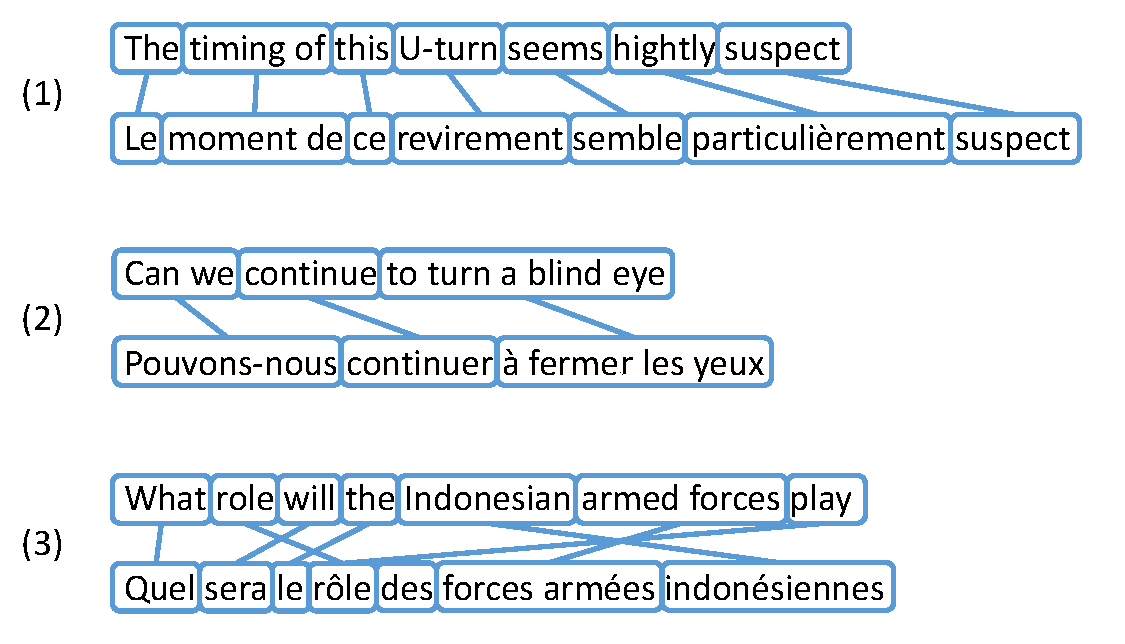
\includegraphics[width=0.8\linewidth]{figures/Figure_goodAli1}
\newcolumntype{C}{>{\centering\arraybackslash} m{10.cm} }
\begin{tabular}{lC}
(1) & 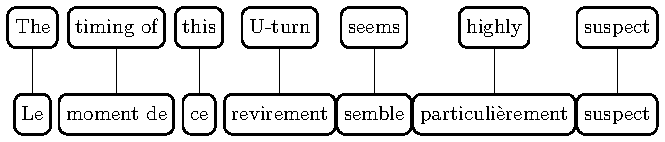
\includegraphics[scale=.9]{figures/figSemmar} \\[1ex]
(2) & 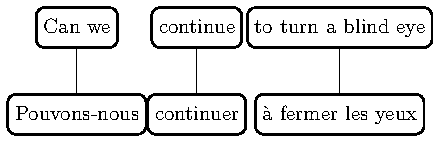
\includegraphics[scale=.9]{figures/figSemmar2}\\[1ex]
(3) & 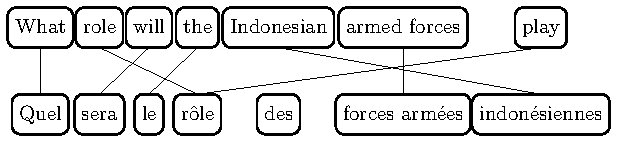
\includegraphics[scale=.9]{figures/figSemmar3}\\
\end{tabular}
\caption{\label{sem:fig:goodali}Good alignments with co-occurrence based metric}
\end{figure}

\begin{figure}
\centering
%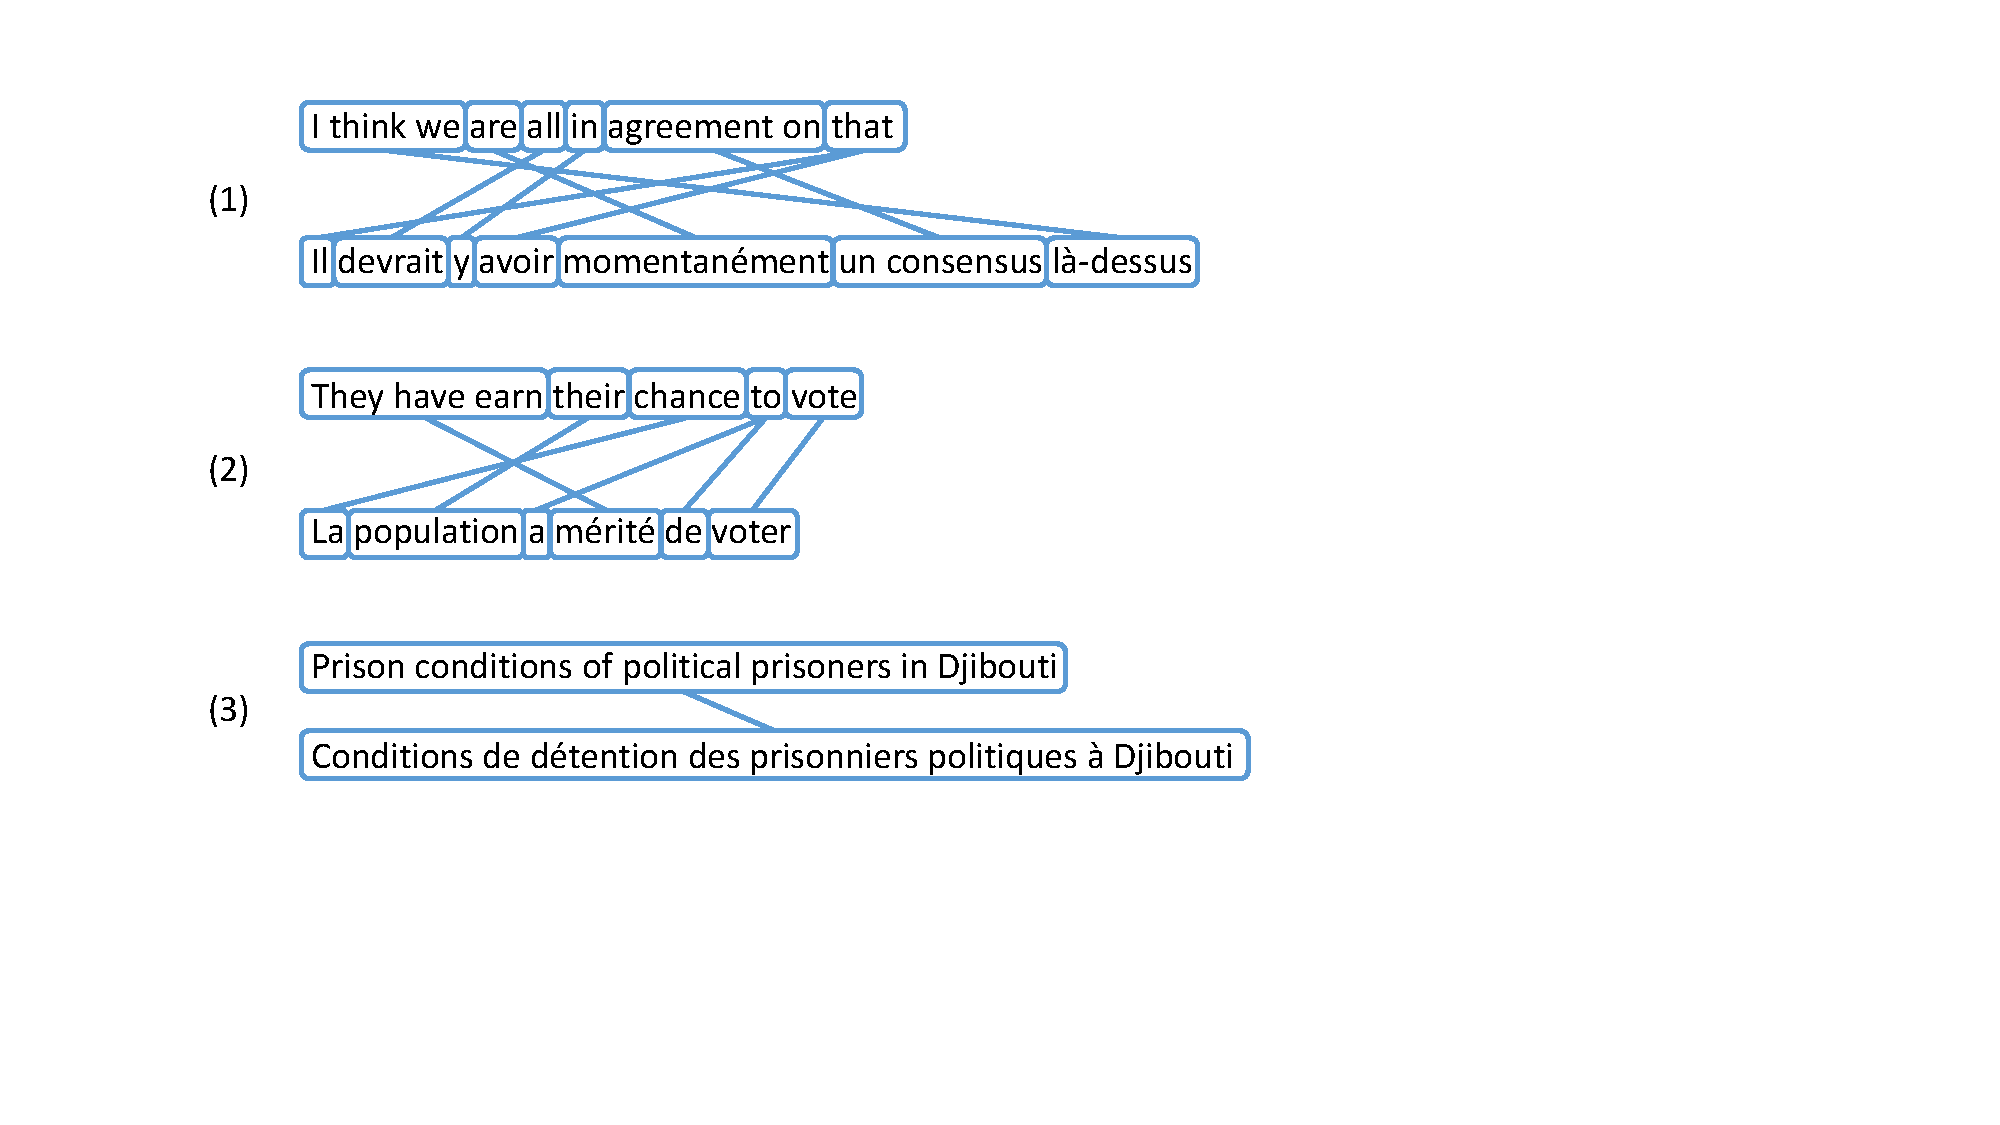
\includegraphics[width=0.75\linewidth]{figures/Figure_badAli}
\newcolumntype{C}{>{\centering\arraybackslash} m{10.cm} }
\begin{tabular}{lC}
(1) & 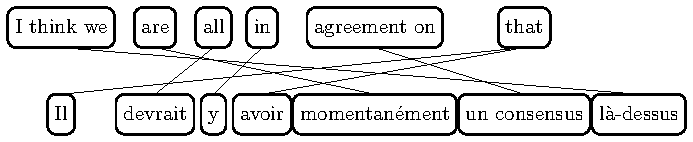
\includegraphics[scale=.9]{figures/figSemmar4} \\[1ex]
(2) & 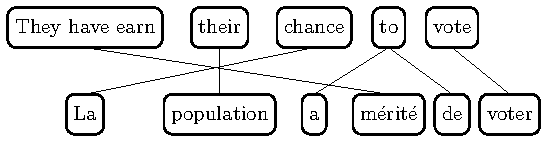
\includegraphics[scale=.9]{figures/figSemmar5} \\[1ex]
(3) & 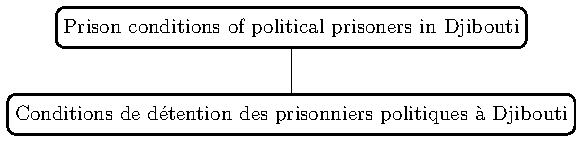
\includegraphics[scale=.9]{figures/figSemmar6} \\
\end{tabular}
\caption{\label{sem:fig:badali}Bad alignments with co-occurrence based metric}
\end{figure}

We also observe that, for common words, the distribution of apparition is meaningless: ``to'' is linked with ``de'' and ``a''. 
We should use a measure of information as suggested in \citet{gao1998automatic}.
In addition, the program is powerless if it finds an unknown word or if a word co-occurs with no other word of the translated sentence. 
In that case, all links containing this word will obtain the score of 0 as they never occur. 
And as we use a multiplicative metric, the global score of the \isi{alignment} will be 0 whatever the other links of the \isi{alignment}. Unknown links should have a small, non-null score to allow the discovery of new links. 
Moreover, we can use an external resource such as a \isi{bilingual lexicon} of single words which can improve the \isi{alignment} of phrases.


\subsubsection{Bilingual dictionary based metric}

The bilingual dictionary gives us several word-to-word alignments. We want to comply with these alignments as often as possible as we infer that they are mostly correct. %(We consider \isi{alignment} only for plain words, not function words).
The dictionary also gives negative \isi{alignment} information. Of course if two words are not aligned by the dictionary we cannot take for sure that they should not. But we have to take that into account.

The bilingual dictionary score is calculated as follows:

\begin{equation}
\phi_c(e_{ij},f_{kl})=\frac{a\times R_1 + b\times R_0}{a\times R_1 + b\times R_0 + c\times N_1 + d\times N_0}
\end{equation}

$R_1$ is the number of respected links, $R_0$ is the number of respected non-links, $N_1$ is the number of non-respected links, and $N_0$ is the number of non-respected non-links.

The coefficients \textit{a}, \textit{b}, \textit{c} and \textit{d} can be adapted to balance the relative influence of the four terms. 
We analyzed a small corpus that allowed us to empirically choose the use of the following values:  \textit{a} = \textit{b} = \textit{c} = 1 and \textit{d} = 0.5. 
The score is calculated for each part of the bi-\isi{phrase} and then the two of them are multiplied. We have to take into account $R_0$ and $N_0$ because otherwise the whole bi-sentence would be the optimal segmentation.

As we can see, this metric has a double effect. 
First, it gives a high score if bi-phrases respect dictionary word to \isi{word alignment}. 
And second, due to $R_0$, it sets a threshold score for unknown couples. 
Both effects can have a positive role in \isi{alignment} task as we will see in the following examples. The dictionary-based metric is not intended to be used separately. It is mixed with 
co-occurrence score. We used an \ili{English}-\ili{French} bilingual dictionary containing 243,539 entries with doubles.\footnote{\url{http://catalog.elra.info/product_info.php?products_id=666.}}

\begin{figure}
\centering
%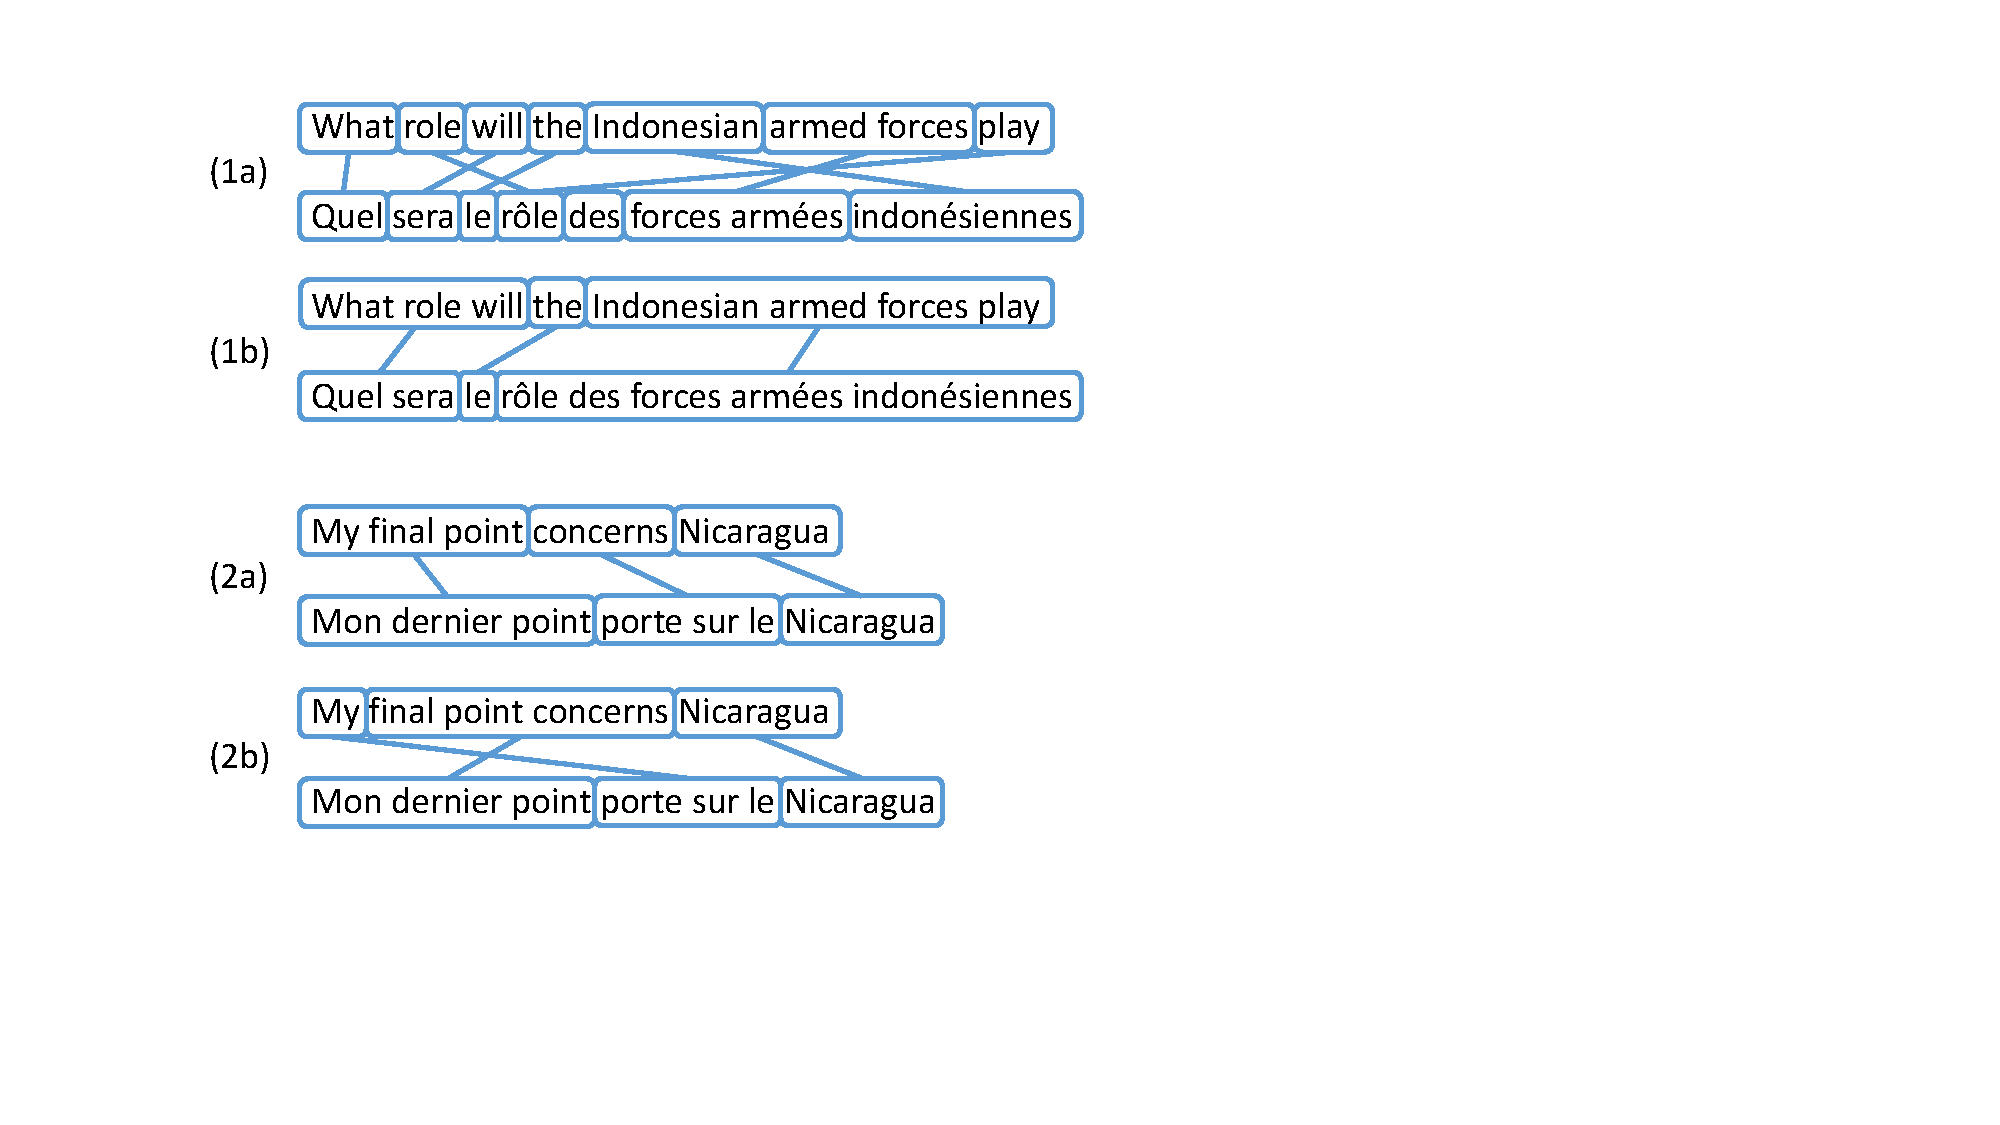
\includegraphics[width=0.7\linewidth]{figures/Figure_degAli}
\newcolumntype{C}{>{\centering\arraybackslash} m{9.cm} }
\begin{tabular}{lC}
(1a) & 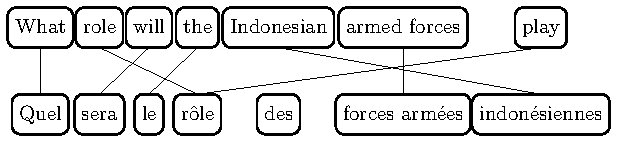
\includegraphics[scale=.9]{figures/figSemmar3}\\[1ex]
(1b) & 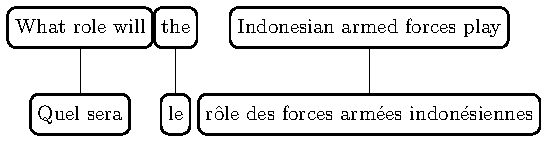
\includegraphics[scale=.9]{figures/figSemmar7}\\[2ex]
(2a) & 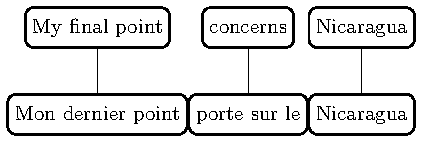
\includegraphics[scale=.9]{figures/figSemmar8}\\[1ex]
(2b) & 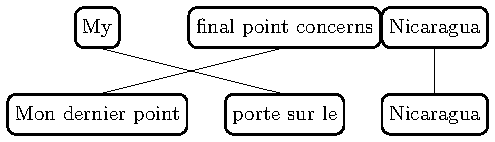
\includegraphics[scale=.9]{figures/figSemmar9}\\
\end{tabular}
\caption{\label{sem:fig:degali}Degradation of alignments - (a) Alignments without the bilingual dictionary and (b) Alignments with the bilingual dictionary}
\end{figure}

\begin{figure}
  \centering
  %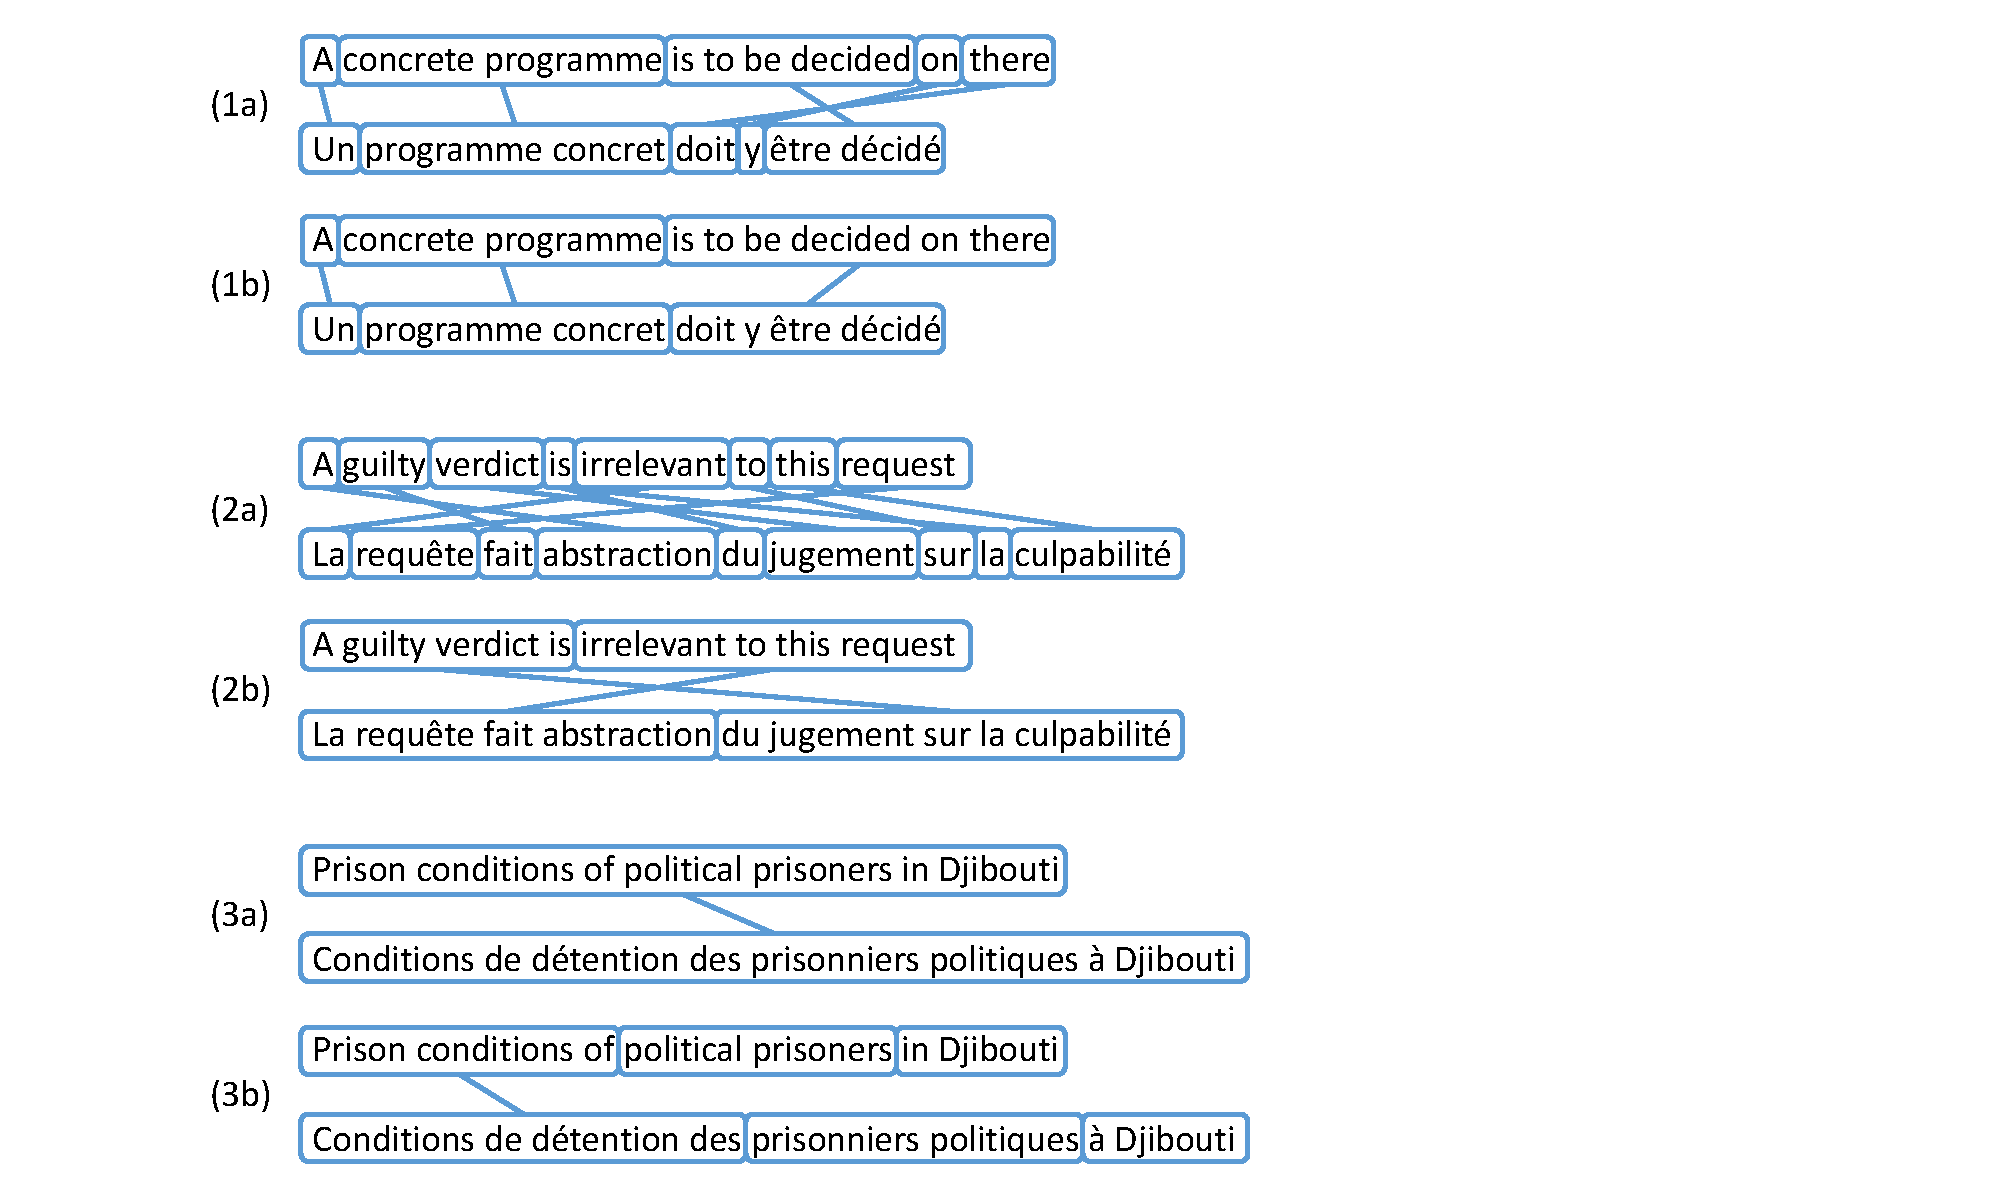
\includegraphics[width=0.85\linewidth]{figures/Figure_impAli-}
  \newcolumntype{C}{>{\centering\arraybackslash} m{.95\textwidth} }
  \begin{tabular}{l@{}C}
    (1a) & 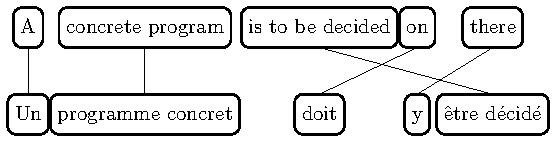
\includegraphics[scale=.85]{figures/figSemmar10}\\[1ex]
    (1b) & 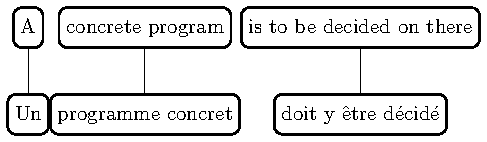
\includegraphics[scale=.85]{figures/figSemmar11}\\[2ex]
    (2a) & 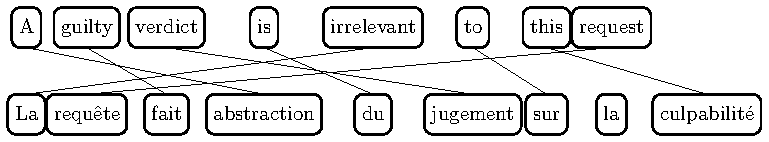
\includegraphics[scale=.85]{figures/figSemmar12}\\[1ex]
    (2b) & 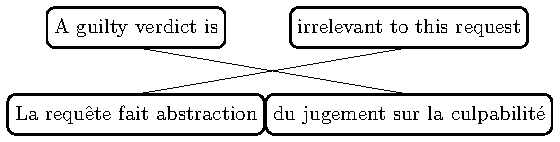
\includegraphics[scale=.85]{figures/figSemmar13}\\[2ex]
    (3a) & 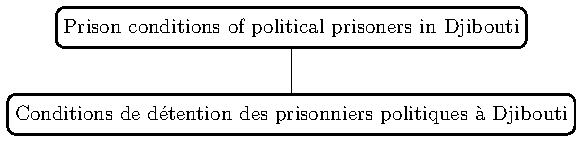
\includegraphics[scale=.85]{figures/figSemmar14}\\[1ex]
    (3b) & 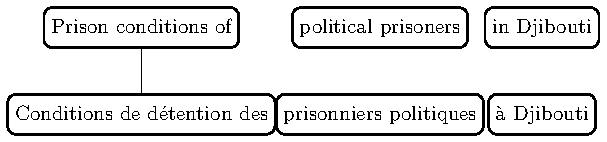
\includegraphics[scale=.85]{figures/figSemmar15}\\
  \end{tabular}
  \caption{\label{sem:fig:improvali}Amelioration of alignments - (a) Alignments without the bilingual dictionary and (b) Alignments with the bilingual dictionary}
\end{figure}


In Figure~\ref{sem:fig:degali}, we observe some degradation of alignments.
For these sentences, the threshold for unknown couples is too high relatively to the statistical score. 
So we lose the benefit of the \isi{co-occurrence metric}. 
This problem should be partially solved by scaling the two metrics. However we have already observed some improvements, as presented in Figure~\ref{sem:fig:improvali}. In the first example, the bilingual dictionary gives the alignments: ``be/être'', ``decided/décidé'' and ``there/y''. So the program manages to reconstruct the whole expression ``is to be decided on there/doit y être décidé''. Moreover the links ``concrete/concret'' and ``programme/programme'' are strengthened. The second example is difficult to align due to the difference of structure. The \isi{alignment} with dictionary is not perfect but is far more better. In this case the dictionary only gives links ``verdict/jugement'' and ``request/requête'' which were already aligned. However they are strengthened and others links are weakened. That is why we can observe an improvement.

Finally in the last example, the dictionary gives no links because the words are not lemmatized. The good result is here exclusively due to the threshold effect. The programme is allowed to consider links with no co-occurrence as long as others links have a good co-occurrence score.


% Experimental results
\section{Experimental results}
The quality of \isi{alignment} of MWEs and the impact of using MWEs on machine translation have been evaluated, firstly, manually, by comparing the results of the three MWEs aligners with a reference \isi{alignment};
and secondly automatically by using the results of the three MWEs aligners to build the \isi{translation model} of the state-of-the-art \isi{statistical machine translation} system Moses \citep{koehn2007moses}.


\subsection{Manual evaluation}

The three approaches for MWEs \isi{alignment} and the baseline Giza++ \citep{och2000improved} have been evaluated using the following evaluation metrics. 
Given an \isi{alignment} A, and a gold standard \isi{alignment} (reference \isi{alignment}) G, each such \isi{alignment} set eventually consisting of two sets $(A_s, A_p)$, and $(G_s, G_p)$ where ``s'' and ``p'' correspond respectively to ``Sure'' and ``Probable'' alignments. 
The following measures are defined (where T is the \isi{alignment} type, and can be set to either S or P). Each word aligner was evaluated in terms of Precision ($P_T$), Recall ($R_T$) and F-Measure ($F_T$).
\begin{equation}
P_T=\frac{A_T \cap G_T}{A_T} ;~
R_T=\frac{A_T \cap G_T}{G_T} ;~
F_T=\frac{2 \times P_T \times R_T}{P_T + R_T}
\label{sem:equa:PRF}
\end{equation}

The corpus used to evaluate the performance of the \ili{English}-\ili{French} MWE aligners is composed of a set of 1992 parallel sentences extracted from Europarl (European Parliament Proceedings). This parallel corpus is composed of 46265 \ili{English} words and 49332 \ili{French} words and has been used to build manually the reference \isi{alignment} by the Yawat tool (Germann, 2008).

Table~\ref{sem:tab:resultsPRF_en-fr} summarizes the results of the three approaches for \ili{English}--\ili{French} MWEs alignments and the baseline (Giza++) in terms of precision, recall and f-measure.

\begin{table}
\caption{Performance of the different English--French MWE aligners}
\label{sem:tab:resultsPRF_en-fr}
 \begin{tabular}{p{6.5cm}ccc}
  \lsptoprule
            \textnormal{MWE aligner} & \textnormal{precision} & \textnormal{recall} & \textnormal{f-measure} \\
  \midrule
Baseline (Giza++) & 0.83 & 0.37 & 0.51 \\
Statistical & 0.81 & 0.39 & 0.52 \\
Hybrid using morpho-syntactic patterns & 0.87 & 0.55 & 0.67 \\
Hybrid using co-occurrence & 0.61 & 0.63 & 0.61 \\
Hybrid using co-occurrence + lexicon & 0.85 & 0.54 & 0.66 \\
  \lspbottomrule
 \end{tabular}
\end{table}



The first observation is that, the hybrid approach based on morpho-syntactic patterns performs better than all the other methods. It clearly appears that the morpho-syntactic patterns used to extract the MWEs present in source and target texts has had a significant impact on the precision of the \isi{alignment}. On the other hand, the statistical approach has the lower recall but it is better than the recall of the baseline (Giza++). And as a second observation, adding information coming from a \isi{bilingual lexicon} to the \isi{co-occurrence metric} used in the hybrid approach based on \isi{linear programming}, certainly has improved the precision but the recall has dropped.

\subsection{Alignment evaluation through a translation task}

The unavailability of a reference \isi{alignment} of a significant size for MWEs does not allow us to achieve a large evaluation and to compare our approaches with the state-of-the-art work. That's why we decided to study the impact of MWEs on the quality of translation by integrating the results of our word aligners in the training corpus used to extract the \isi{translation model} of the \isi{phrase} based \isi{statistical machine translation} system Moses. We use the factored \isi{translation model} \citep{koehn2007factored} as our baseline system. It is an extension of the \isi{phrase} based models which are limited to the mappings of phrases without any explicit use of linguistic information.  The factored model enables the use of additional markup at the word level (Figure~\ref{sem:fig:factModel}).

\begin{figure}
\centering
%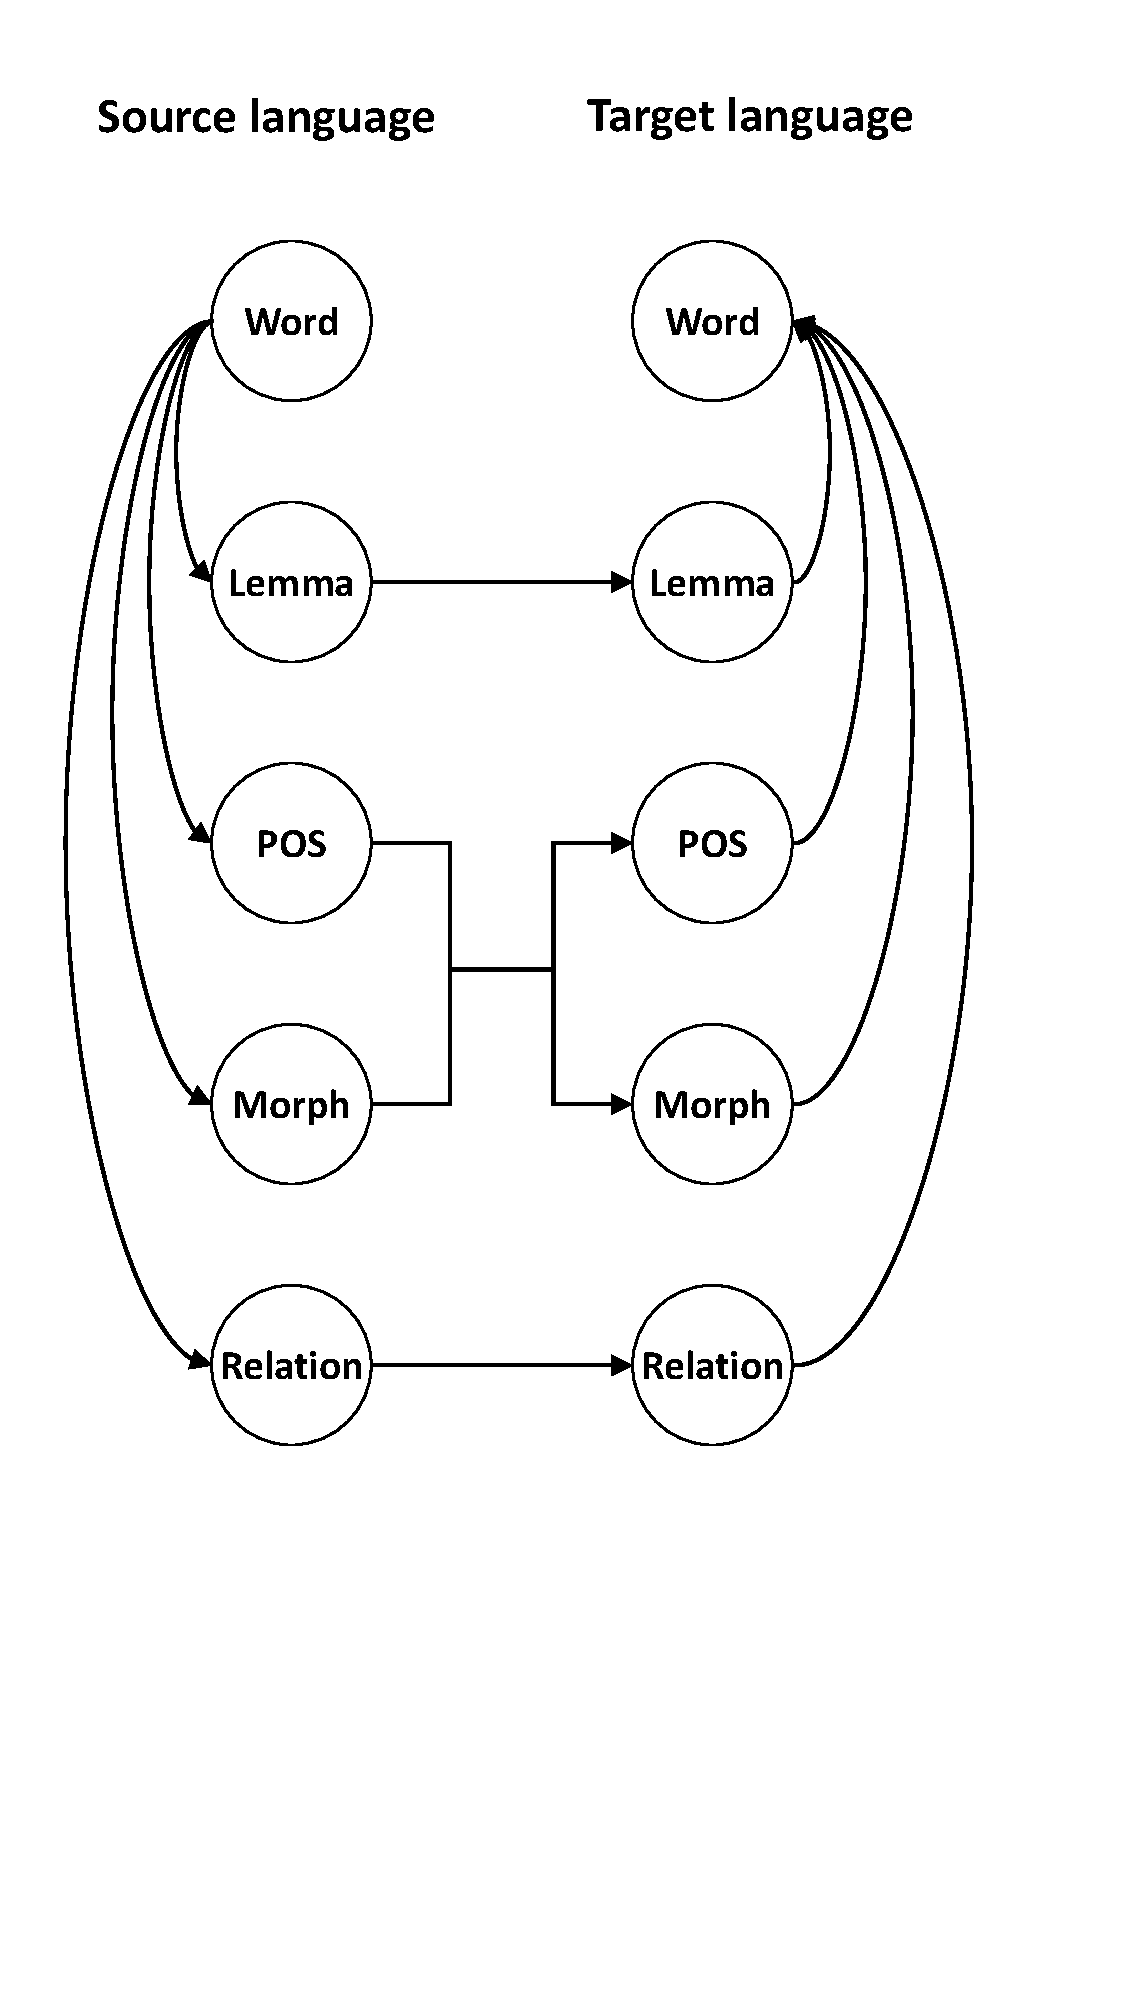
\includegraphics[width=0.5\linewidth]{figures/Figure_FactTrans_NB}

\tikzset{
    %Define standard arrow tip
    >=stealth',
    %Define style for boxes
    punkt/.style={
           circle,
           draw=black, very thick,
           text width=3.2em,
           %minimum height=2em,
           text centered},
}
\resizebox{.7\textwidth}{!}{%
  \begin{tikzpicture}[node distance=1cm]
    %nodes
    \node[punkt] (word) {Word};
    \node[punkt, inner sep=5pt,below=0.5cm of word]
    (lemma) {Lemma};
    \node[punkt, inner sep=5pt,below=0.5cm of lemma]
    (pos) {POS};
    \node[punkt, inner sep=5pt,below=0.5cm of pos]
    (morph) {Morph};
    \node[punkt, inner sep=5pt,below=0.5cm of morph]
    (relation) {Relation};
    
    \node[right=.5cm of pos] (empty1) {}; 
    \node[below=.8cm of empty1] (empty2) {};

    \node[punkt, right=2.3cm of word] (wordT) {Word};
    \node[punkt, inner sep=5pt,below=0.5cm of wordT]
    (lemmaT) {Lemma};
    \node[punkt, inner sep=5pt,below=0.5cm of lemmaT]
    (posT) {POS};
    \node[punkt, inner sep=5pt,below=0.5cm of posT]
    (morphT) {Morph};
    \node[punkt, inner sep=5pt,below=0.5cm of morphT]
    (relationT) {Relation};
    
    \node[left=.5cm of posT] (empty1T) {}; 
    \node[below=.8cm of empty1T] (empty2T) {};
    
    % We make a dummy figure to make everything look nice.
    \node[above=.5cm of word] (source) {Source language};
    \node[right=of source] (target) {Target language};
    
    \draw[->, >=latex] (lemma) -- (lemmaT);
    \draw[->, >=latex] (relation) -- (relationT);
    
    \draw[>=latex] (pos) -| (empty2.center);
    \draw[>=latex] (morph) -| (empty2.center); 
    
    \draw[<-,>=latex] (posT) -| (empty2T.center);
    \draw[<-,>=latex] (morphT) -| (empty2T.center); 
    
    \draw[>=latex] (empty2.center) -- (empty2T.center); 
    
    \draw[->, >=latex] (word.west) to[bend right=45] (lemma.west) ;
    \draw[->, >=latex] (word.west) to[bend right=45] (pos.west) ;
    \draw[->, >=latex] (word.west) to[bend right=45] (morph.west) ;
    \draw[->, >=latex] (word.west) to[bend right=45] (relation.west) ;  
    
    \draw[<-, >=latex] (wordT.east) to[bend left=45] (lemmaT.east) ;
    \draw[<-, >=latex] (wordT.east) to[bend left=45] (posT.east) ;
    \draw[<-, >=latex] (wordT.east) to[bend left=45] (morphT.east) ;
    \draw[<-, >=latex] (wordT.east) to[bend left=45] (relationT.east) ;  
  \end{tikzpicture}
}

\caption{\label{sem:fig:factModel}Factored model used in the SMT baseline system}
\end{figure}

Our model operates on lemmas instead of surface forms, in which the translation process is broken up into a sequence of mapping steps that either:
\begin{itemize}
\item Translate source lemmas into target's ones.
\item Generate surface forms given the lemma.
\end{itemize}


The features used in the baseline system include: (1) four translation probability features, (2) two language models, (3) one generation model and (4) word penalty. %For the CORPUS method, bilingual MWEs are added into the training corpus, as result, new \isi{alignment} and \isi{phrase} table are obtained. 

The goal of these experiments is to study in what respect MWEs are useful to improve the performance of Moses. In Moses, \isi{phrase} tables are the main knowledge source for the machine translation decoder. The decoder consults these tables to figure out how to translate an input sentence into the target language. These tables are built automatically using the open source \isi{word alignment} tool Giza++ \citep{och2000improved}. However, Giza++ could produce errors in particular when it aligns multiword expressions \citep{fraser2007measuring}. In order to integrate into Moses the \isi{bilingual lexicon} which is extracted automatically by the \isi{MWE alignment} approaches, we propose the following three methods:
\begin{description}
\item[CORPUS:] In this method, we add the extracted \isi{bilingual lexicon} as a parallel corpus and retrain the \isi{translation model}. By increasing the occurrences of the MWEs and their translations, we expect a modification of \isi{alignment} and probability estimation.
 \item[TABLE:] This method consists in adding the extracted \isi{bilingual lexicon} into Moses’s \isi{phrase} table. We use a smoothed probability estimator to construct a translation probability for each MWE of the \isi{bilingual lexicon}. This estimator is based on the similarity measure provided by each \isi{word alignment} approach.
 \item[FEATURE:] In this method, we extend the ``TABLE'' method by adding a new feature indicating whether a MWE comes from the \isi{bilingual lexicon} or not (l or 0 is introduced for each entry of the \isi{phrase} table).
\end{description}



\subsubsection{Data and experimental setup}
In order to study the impact of the \isi{bilingual lexicon} of MWEs on the performance of Moses, we conducted our experiments on two \ili{English}-\ili{French} \isi{parallel corpora} (Table~\ref{sem:tab:data}): Europarl (European Parliament Proceedings) and Emea (European Medicines Agency Documents). These corpora were extracted from the open parallel corpus OPUS \citep{tiedemann2012parallel}. For each \isi{MWE alignment} approach, we achieved three runs and two test experiments for each run: In-Domain and Out-Of-Domain. For this, we randomly extracted 500 parallel sentences from Europarl as an In-Domain corpus and 500 pairs of sentences from Emea as Out-Of-Domain corpus. The \isi{domain vocabulary} is represented in the case of our baseline (Moses) respectively by the specialized parallel corpus Emea which is added to the training data (Europarl). Afterwards, we extracted bilingual MWEs from the training corpus and applied the three methods described above. For the three integration methods (CORPUS, TABLE, FEATURE), the \isi{domain vocabulary} is identified by a \isi{bilingual lexicon} which is extracted automatically from the specialized parallel corpus Emea using the different MWEs \isi{alignment} approaches.

\begin{table}
\caption{Europarl and Emea corpora details used to train language and translation models of Moses (K refers to $10^3$)}
\label{sem:tab:data}
%\scriptsize
\centering
 \begin{tabular}{lcc} 
  \lsptoprule
  Run n°. & Training (\# sentences) & Tuning (\# sentences) \\
  \midrule
1 & 150K+10K (Europarl+Emea) & 2K+0.5K (Europarl+Emea)\\
2 & 150K+20K (Europarl+Emea) & 2K+0.5K (Europarl+Emea)\\
3 & 150K+30K (Europarl+Emea) & 2K+0.5K (Europarl+Emea)\\
  \lspbottomrule
 \end{tabular}
\end{table}


\subsubsection{Results and discussion}
The performance of the SMT system Moses is evaluated using the BLEU score \citep{papineni2002bleu} on the two test sets for the three runs described in the previous section. 
Note that we consider one reference per sentence. The obtained results are reported in tables~\ref{sem:tab:SMT1},~\ref{sem:tab:SMT2},~\ref{sem:tab:SMT3} and~\ref{sem:tab:SMT4}.

\begin{table}
\caption{BLEU scores of Moses when using the results of the statistical approach}
\label{sem:tab:SMT1}
\fittable{%
\scriptsize
\centering
 \begin{tabular}{lcccccccc} 
  \lsptoprule
  Run n°. & \multicolumn{4}{c}{In-Domain (Europarl)} & \multicolumn{4}{c}{Out-Of-Domain (Emea)} \\
 & Baseline & CORPUS & TABLE & FEATURE & Baseline & CORPUS & TABLE & FEATURE \\
  \midrule
1 & 32.62 & 32.41 & 32.36 & 32.55 & 22.96 & 22.82 & 22.75 & 22.91 \\
2 & 33.81 & 33.76 & 33.71 & 33.79 & 23.30 & 23.09 & 23.04 & 23.27 \\
3 & 34.25 & 34.23 & 34.21 & 34.24 & 24.55 & 24.49 & 24.45 & 24.52 \\
  \lspbottomrule
 \end{tabular}
 }
\end{table}

\begin{table}
\caption{BLEU scores of Moses when using the results of the hybrid approach based on morpho-syntactic patterns}
\fittable{%
\scriptsize
\centering
\label{sem:tab:SMT2}
 \begin{tabular}{lcccccccc} 
  \lsptoprule
  Run n°. & \multicolumn{4}{c}{In-Domain (Europarl)} & \multicolumn{4}{c}{Out-Of-Domain (Emea)} \\
 & Baseline & CORPUS & TABLE & FEATURE & Baseline & CORPUS & TABLE & FEATURE \\
  \midrule
1 & 32.62 & 32.82 & 32.15 & 32.88 & 22.96 & 23.45 & 23.11 & 23.69 \\
2 & 33.81 & 34.05 & 33.48 & 34.09 & 23.30 & 24.09 & 23.76 & 24.18 \\
3 & 34.25 & 34.64 & 34.11 & 34.67 & 24.55 & 25.43 & 25.05 & 25.48 \\
  \lspbottomrule
 \end{tabular}
 }
\end{table}

\begin{table}
\caption{BLEU scores of Moses when using the results of the hybrid approach based on linear programming}
\fittable{%  
\scriptsize
\centering
\label{sem:tab:SMT3}
 \begin{tabular}{lcccccccc} 
  \lsptoprule
  Run n°. & \multicolumn{4}{c}{In-Domain (Europarl)} & \multicolumn{4}{c}{Out-Of-Domain (Emea)} \\
 & Baseline & CORPUS & TABLE & FEATURE & Baseline & CORPUS & TABLE & FEATURE \\
  \midrule
1 & 32.62 & 32.69 & 32.64 & 32.72 & 22.96 & 23.03 & 22.97 & 23.06 \\
2 & 33.81 & 33.88 & 33.85 & 33.91 & 23.30 & 23.37 & 23.34 & 23.40 \\
3 & 34.25 & 34.30 & 34.27 & 34.33 & 24.55 & 24.59 & 24.56 & 24.62 \\
  \lspbottomrule
 \end{tabular}
 }
\end{table}

\begin{table}

\caption{BLEU scores of Moses when using the results of the hybrid approach based on linear programming and using a bilingual dictionary}
\label{sem:tab:SMT4}
\fittable{%
\scriptsize
\centering
 \begin{tabular}{lcccccccc} 
  \lsptoprule
  Run n°. & \multicolumn{4}{c}{In-Domain (Europarl)} & \multicolumn{4}{c}{Out-Of-Domain (Emea)} \\
 & Baseline & CORPUS & TABLE & FEATURE & Baseline & CORPUS & TABLE & FEATURE \\
  \midrule
1 & 32.62 & 32.71 & 32.68 & 32.73 & 22.96 & 23.06 & 22.97 & 23.07 \\
2 & 33.81 & 33.89 & 33.87 & 33.92 & 23.30 & 23.39 & 23.32 & 23.39 \\
3 & 34.25 & 34.32 & 34.29 & 34.32 & 24.55 & 24.62 & 24.56 & 24.63 \\
  \lspbottomrule
 \end{tabular}
 }
\end{table}

As shown in tables 6, 7, 8 and 9, for In-Domain texts, Moses achieve a relatively high BLEU score and the scores of Moses when using the results of the hybrid approach based on morpho-syntactic patterns are better in all the runs. The best improvement is achieved using the ``FEATURE'' method. %This method (when compared to the baseline system) reports a gain of +0.42 points in BLEU score for In-Domain texts and +0.93 points for the Out-Of-Domain sentences (Table 7, Run 3).
The ``CORPUS''method (when compared to the baseline system) comes next with a slightly higher BLEU score with an improvement %of +0.39 points
for In-Domain sentences and %+0.88 points for the
Out-Of-Domain texts.

In order to show the impact of the \isi{domain vocabulary} (represented by the bilingual MWEs extracted with the aligner based on the hybrid approach with morpho-syntactic patterns), on the \isi{translation quality} of Moses, we manually analyzed an example of translations drawn from the Out-Of-Domain test corpus (Table 11).

\begin{table}
\caption{Translations produced by Moses for an Out-Of-Domain sentence}
\label{sem:tab:SMT_ex2}
\small
\centering
 \begin{tabular}{p{0.3\linewidth}p{0.6\linewidth}} 
  \lsptoprule
Input sentence & in the 12 week acute phase of three clinical trials of duloxetine in patients with diabetic neuropathic pain, small but statistically significant increases in fasting blood glucose were observed in duloxetine-treated patients. \\
  \midrule
Reference translation & lors de la phase aiguë de 12 semaines de trois essais cliniques étudiant la duloxétine chez les patients souffrant de douleur neuropathique diabétique, des augmentations faibles, mais statistiquement significatives de la glycémie à jeun ont été observées chez les patients sous duloxétine. \\
  \midrule
Moses translation with the ``CORPUS'' integration method & dans le 12 semaines de la phase aiguë trois études cliniques de duloxetine chez les patients avec douleur neuropathique diabétique, petites mais statistiquement significatif augmentations de répréhensible glycémie artérielle a été observée chez les patients traités duloxetine.\\
  \midrule
Moses translation with the ``TABLE'' integration method & dans le 12 semaine de la phase aiguë de trois essais cliniques de duloxetine dans les patients avec douleur neuropathique diabétique, petites mais statistiquement augmentations considérables dans le sang répréhensible glucose ont été constatées dans les patients duloxetine traités.\\
  \midrule
Moses translation with the ``FEATURE'' integration method & dans le 12 semaines de la phase aiguë de trois essais cliniques chez les patients avec douleur neuropathique diabétique, petites mais des augmentations statistiquement significatives de la glycémie à jeun ont été observées chez les patients traités duloxétine.\\
  \lspbottomrule
 \end{tabular}
\end{table}

After analyzing the translations of this example, it is clear that in some cases, it is just impossible to perform a word-to-\isi{word alignment} between two MWEs that are translation of each other. For example, the ``FEATURE'' method proposes the \isi{compound word} “glycémie à jeun” as a translation for the expression “fasting blood glucose” which is correct, but, ``CORPUS'' and ``TABLE'' methods propose respectively the translations “répréhensible glycémie artérielle” and “sang répréhensible glucose” which are completely wrong. However, all the integration methods translate correctly the multiword expressions “diabetic neuropath\-ic pain/douleur neuropathique diabétique” and “acute phase/phase aiguë”. The multiword expression “clinical trials/essais cliniques” is translated correctly by ``TABLE'' and ``FEATURE'' methods. Likewise, the translation provided by the ``CORPUS'' method for this expression is also correct “clinical trials/études cliniques” but it is different from the translation of the reference. It seems that the probabilities of the alignments proposed by Giza++ for these multiword expressions were very high and helped Moses decoder to choose these alignments. On the other hand, as we can see, all the translations have many spelling and grammatical errors, and in particular, the translations of some multiword expressions (statistically significant increases/\textit{statistiquement significatif augmentations}, statistically significant increases/\textit{statistiquement augmentations considérables}) produced by the ``CORPUS'' and ``TABLE'' methods are very approximate. This result can be explained by the fact that, on the one hand, \isi{statistical machine translation} toolkits like Moses have not been designed with grammatical error correction in mind, and on the other hand, Giza++ could produce errors in particular when it aligns multiword expressions  \citep{fraser2007measuring}. For the multiword expression “duloxetine-treated patients”, the methods ``FEATURE'' and ``CORPUS'' provide a same translation which is more or less correct (``patients traités duloxetine''). However, the method TABLE provides a translation in a poor \isi{grammar} (``patients duloxetine traités'').

Finally on this point, we can observe that the major issues of Moses concern errors produced by Giza++ when aligning multiword expressions (\isi{translation model}), and incorrect spelling and poor \isi{grammar} generated by the decoder (language model). To handle the first issue, we proposed to take into account the specialized \isi{bilingual lexicon} extracted with the MWEs aligner into Moses’s \isi{phrase} table and we added a new feature indicating whether a word comes from this lexicon or not (FEATURE method). However, for spelling and \isi{grammar} errors, Moses has no specific treatment.

\section{Conclusion and future work}

We have described, in this chapter, three approaches aiming to extract and align MWEs in \ili{English}-\ili{French} \isi{parallel corpora}. We have also presented an experimental evaluation of the impact of integrating the results of these MWEs \isi{alignment} approaches on the performance of the \isi{statistical machine translation} system Moses. We have more specifically shown that, on the one hand, the hybrid approach based on morpho-syntactic patterns performs better than the other approaches and the ``FEATURE'' integration method achieves the best improvement, and on the other hand, using MWEs as additional parallel sentences to train the \isi{translation model} of Moses improves its BLEU score.

This study offers several open issues for future work. First, we should explore machine learning approaches to extend the morphosyntactic patterns to take into account other forms of MWEs. The second perspective is to explore the integration of bilingual MWEs into other machine translation models such as rule-based translation ones. We also expect to explore the use of LSTM (Long Short-Term Memory) recurrent neural network language models for rescoring the n-best translations produced by Moses in order to reduce \isi{grammar} errors.


% \section{Where we came from} 
% Phasellus maximus erat ligula, accumsan rutrum augue facilisis in. Proin sit amet pharetra nunc, sed maximus erat. Duis egestas mi eget purus venenatis vulputate vel quis nunc. Nullam volutpat facilisis tortor, vitae semper ligula dapibus sit amet. Suspendisse fringilla, quam sed laoreet maximus, ex ex placerat ipsum, porta ultrices mi risus et lectus. Maecenas vitae mauris condimentum justo fringilla sollicitudin. Fusce nec interdum ante. Curabitur tempus dui et orci convallis molestie \citep{Chomsky1957}.

% \begin{table}
% \caption{Frequencies of word classes}
% \label{sem:tab:1:frequencies}
%  \begin{tabular}{lllll} 
%   \lsptoprule
%             & nouns & verbs & adjectives & adverbs\\ 
%   \midrule
%   absolute  &   12 &    34  &    23     & 13\\
%   relative  &   3.1 &   8.9 &    5.7    & 3.2\\
%   \lspbottomrule
%  \end{tabular}
% \end{table}

% Sed nisi urna, dignissim sit amet posuere ut, luctus ac lectus. Fusce vel ornare nibh. Nullam non sapien in tortor hendrerit suscipit. Etiam sollicitudin nibh ligula. Praesent dictum gravida est eget maximus. Integer in felis id diam sodales accumsan at at turpis. Maecenas dignissim purus non libero scelerisque porttitor. Integer porttitor mauris ac nisi iaculis molestie. Sed nec imperdiet orci. Suspendisse sed fringilla elit, non varius elit. Sed varius nisi magna, at efficitur orci consectetur a. Cras consequat mi dui, et cursus lacus vehicula vitae. Pellentesque sit amet justo sed lectus luctus vehicula. Suspendisse placerat augue eget felis sagittis placerat. 

% \ea
% \gll cogito                           ergo      sum\\  
%      think.\textsc{1sg}.\textsc{pres} therefore \textsc{cop}.\textsc{1sg}.\textsc{pres}\\ 
% \glt `I think therefore I am.'
% \z

% Sed cursus eros condimentum mi consectetur, ac consectetur sapien pulvinar. Sed consequat, magna eu scelerisque laoreet, ante erat tristique justo, nec cursus eros diam eu nisl. Vestibulum non arcu tellus. Nunc dignissim tristique massa ut gravida. Nullam auctor orci gravida tellus egestas, vitae pharetra nisl porttitor. Pellentesque turpis nulla, venenatis id porttitor non, volutpat ut leo. Etiam hendrerit scelerisque luctus. Nam sed egestas est. Suspendisse potenti. Nunc vestibulum nec odio non laoreet. Proin lacinia nulla lectus, eu vehicula erat vehicula sed. 


% \section*{Abbreviations}
% \section*{Acknowledgements}

\printbibliography[heading=subbibliography,notkeyword=this]
% \bibliographystyle{langsci-unified}
% \bibliography{main-blx}
\end{document}
